\chapter{Additional Data}
\section{Code-to-code Verification Between SAPHIRE and SCRAM}
\label{sec:appendix_a}

Before running benchmark tests to compare the execution runtimes and memory usage of SAPHSOLVE and SCRAM, it is essential to perform a code-to-code verification to ensure both solvers produce consistent results. Since SAPHSOLVE (the solver API from SAPHIRE) serves as the source of truth, SCRAM must be verified against it. It should be noted that the current SAPHSOLVE implementation supports only the MOCUS algorithm with the MCUB approximation, whereas SCRAM supports both MCUB and REA approximations with MOCUS, as well as exact quantification using its BDD method.

{
\centering
\footnotesize % Reduces font size
\setlength{\tabcolsep}{3pt} % Reduces space between columns
\begin{longtable}{l S[table-format=7.0] S[table-format=7.0] S[table-format=7.0] S[table-format=10.0] S[table-format=10.0] S[table-format=10.0] S[table-format=5.0]}
\caption{Total number of cut sets per event tree for SAPHSOLVE and SCRAM for different truncation limits.}
\label{tab:number_of_cutsets} \\
\toprule
\multirow{2}{*}{Event Tree} & \multicolumn{3}{c}{Truncation Limit $10^{-12}$} & \multicolumn{3}{c}{Truncation Limit $10^{-20}$} & {Adaptive} \\
\cmidrule(lr){2-4} \cmidrule(lr){5-7}
 & {SAPHSOLVE} & {SCRAM} & {SCRAM-Node} & {SAPHSOLVE} & {SCRAM} & {SCRAM-Node} & {SCRAM-Node} \\
\midrule
\endfirsthead
\multicolumn{8}{c}{\tablename~\thetable: Continued from previous page} \\
\toprule
\multirow{2}{*}{Event Tree} & \multicolumn{3}{c}{Truncation Limit $10^{-12}$} & \multicolumn{3}{c}{Truncation Limit $10^{-20}$} & {Adaptive} \\
\cmidrule(lr){2-4} \cmidrule(lr){5-7}
 & {SAPHSOLVE} & {SCRAM} & {SCRAM-Node} & {SAPHSOLVE} & {SCRAM} & {SCRAM-Node} & {SCRAM-Node} \\
\midrule
\endhead
\midrule
\multicolumn{8}{r}{Continued on next page}\\
\midrule
\endfoot
\bottomrule
\endlastfoot
SGTL-S & 6599 & 6599 & 6599 & 175453 & 175453 & 175453 & 835 \\
PCL & 1429807 & 1429807 & 1429807 & 829656936 & 829656936 & 829656936 & 3987 \\
ATRS & 2387281 & 2387281 & 2387281 & 209644970 & 209644970 & 209644970 & 7126 \\
CRW & 114249 & 114249 & 114249 & 3252341 & 3252341 & 3252341 & 947 \\
LOOP & 2473 & 2473 & 2473 & 43424 & 43424 & 43424 & 113 \\
SGTL-M & 10705 & 10705 & 10705 & 232667 & 232667 & 232667 & 1271 \\
LOHTL & 16130 & 16130 & 16130 & 5357356 & 5357356 & 5357356 & 463 \\
Total & 3967244 & 3967244 & 3967244 & 1048363147 & 1048363147 & 1048363147 & 14742 \\
\end{longtable}
}

The verification compares the two solvers based on (1) the number of cut sets produced and (2) the sequence probability for each event sequence. Table \ref{tab:number_of_cutsets} presents the total cut set counts, while Table \ref{tab:cutsets_merged} details the breakdown for each individual event sequence. The cut set counts from the adaptive quantification method have also been presented in these two tables. These tables summarize the results across three distinct verification scenarios.

First, using a standard truncation limit of $10^{-12}$ and the MOCUS algorithm, the data demonstrates a complete match between the tools for all seven event trees.

Second, the solvers were tested for susceptibility to rounding errors caused by finite precision arithmetic, which can occur when event sequence frequencies are extremely low (on the order of $10^{-20}$). When the truncation limit was lowered to $10^{-20}$, the resulting cut set counts remained consistent between the solvers.

Third, the results validate the model conversion pipeline (JSInp → XML → JSON). As indicated by the matching counts for SCRAM-Node, the translation process preserves the data accurately, and the Node implementation quantifies the results correctly.

{
\centering
\footnotesize % Reduces font size
\setlength{\tabcolsep}{3pt} % Reduces space between columns
\begin{longtable}{l S[table-format=9.0] S[table-format=9.0] S[table-format=9.0] S[table-format=9.0] S[table-format=9.0]}
\caption{Number of cut sets of each sequence for SAPHIRE and SCRAM with different truncation limits.}
\label{tab:cutsets_merged} \\
\toprule
\multirow{2}{*}{Sequence ID} & \multicolumn{2}{c}{Truncation Limit $10^{-12}$} & \multicolumn{2}{c}{Truncation Limit $10^{-20}$} & {Adaptive} \\
\cmidrule(lr){2-3} \cmidrule(lr){4-5}
 & {SAPHSOLVE} & {SCRAM} & {SAPHSOLVE} & {SCRAM} & {SCRAM-Node} \\
\midrule
\endfirsthead
\caption*{Table \thetable{} (continued).}\\
\toprule
\multirow{2}{*}{Sequence ID} & \multicolumn{2}{c}{Truncation Limit $10^{-12}$} & \multicolumn{2}{c}{Truncation Limit $10^{-20}$} & {Adaptive} \\
\cmidrule(lr){2-3} \cmidrule(lr){4-5}
 & {SAPHSOLVE} & {SCRAM} & {SAPHSOLVE} & {SCRAM} & {SCRAM-Node} \\
\midrule
\endhead
\midrule
\multicolumn{6}{r}{Continued on next page}\\
\midrule
\endfoot
\bottomrule
\endlastfoot
S1 & 6 & 6 & 6 & 6 & 5 \\
S2 & 17 & 17 & 19 & 19 & 1 \\
S3 & 0 & 0 & 0 & 0 & 0 \\
S4 & 568 & 568 & 9116 & 9116 & 2 \\
S5 & 2 & 2 & 2 & 2 & 1 \\
S6 & 0 & 0 & 27 & 27 & 24 \\
S7 & 0 & 0 & 0 & 0 & 0 \\
S8 & 0 & 0 & 0 & 0 & 0 \\
S9 & 0 & 0 & 984 & 984 & 42 \\
S10 & 456 & 456 & 3813 & 3813 & 42 \\
S11 & 3 & 3 & 3 & 3 & 3 \\
S12 & 0 & 0 & 0 & 0 & 0 \\
S13 & 4 & 4 & 27 & 27 & 21 \\
S14 & 0 & 0 & 0 & 0 & 0 \\
S15 & 14 & 14 & 918 & 918 & 1 \\
S16 & 529 & 529 & 5354 & 5354 & 1 \\
S17 & 3 & 3 & 3 & 3 & 1 \\
S18 & 9 & 9 & 9 & 9 & 9 \\
S19 & 0 & 0 & 0 & 0 & 0 \\
S20 & 0 & 0 & 671 & 671 & 0 \\
S21 & 4 & 4 & 42521 & 42521 & 337 \\
S22 & 12 & 12 & 664 & 664 & 7 \\
S23 & 9 & 9 & 9 & 9 & 9 \\
S24 & 0 & 0 & 0 & 0 & 0 \\
S25 & 0 & 0 & 2932 & 2932 & 104 \\
S26 & 665 & 665 & 9226 & 9226 & 98 \\
S27 & 25 & 25 & 25 & 25 & 3 \\
S28 & 9 & 9 & 9 & 9 & 9 \\
S29 & 0 & 0 & 0 & 0 & 0 \\
S30 & 0 & 0 & 0 & 0 & 0 \\
S31 & 0 & 0 & 0 & 0 & 0 \\
S32 & 16 & 16 & 28 & 28 & 7 \\
S33 & 0 & 0 & 3502 & 3502 & 50 \\
S34 & 1194 & 1194 & 13290 & 13290 & 50 \\
S35 & 24 & 24 & 28 & 28 & 2 \\
S36 & 49 & 49 & 5296 & 5296 & 1 \\
S37 & 2423 & 2423 & 27250 & 27250 & 1 \\
S38 & 28 & 28 & 28 & 28 & 1 \\
S39 & 0 & 0 & 0 & 0 & 0 \\
S40 & 0 & 0 & 0 & 0 & 0 \\
S41 & 0 & 0 & 0 & 0 & 0 \\
S42 & 0 & 0 & 0 & 0 & 0 \\
S43 & 0 & 0 & 0 & 0 & 0 \\
S44 & 152 & 152 & 1280 & 1280 & 1 \\
S45 & 377 & 377 & 48412 & 48412 & 1 \\
S46 & 1 & 1 & 1 & 1 & 1 \\
S47 & 1 & 1 & 1 & 1 & 1 \\
S48 & 0 & 0 & 375 & 375 & 0 \\
S49 & 0 & 0 & 150711 & 150711 & 403 \\
S50 & 12 & 12 & 8471 & 8471 & 11 \\
S51 & 3 & 3 & 3 & 3 & 2 \\
S52 & 44 & 44 & 257197 & 257197 & 264 \\
S53 & 39858 & 39858 & 1786659 & 1786659 & 264 \\
S54 & 2994 & 2994 & 24218 & 24218 & 10 \\
S55 & 1 & 1 & 1 & 1 & 1 \\
S56 & 1 & 1 & 268 & 268 & 9 \\
S57 & 0 & 0 & 220049 & 220049 & 377 \\
S58 & 2 & 2 & 78154 & 78154 & 34 \\
S59 & 17 & 17 & 6472 & 6472 & 8 \\
S60 & 32 & 32 & 112532 & 112532 & 10 \\
S61 & 2 & 2 & 2 & 2 & 1 \\
S62 & 193 & 193 & 325573 & 325573 & 264 \\
S63 & 151222 & 151222 & 198424900 & 198424900 & 656 \\
S64 & 68314 & 68314 & 1345421 & 1345421 & 57 \\
S65 & 25740 & 25740 & 8296837 & 8296837 & 27 \\
S66 & 3006 & 3006 & 4685 & 4685 & 8 \\
S67 & 40045 & 40045 & 311388 & 311388 & 8 \\
S68 & 1 & 1 & 1 & 1 & 1 \\
S69 & 1 & 1 & 268 & 268 & 9 \\
S70 & 0 & 0 & 253828 & 253828 & 377 \\
S71 & 2 & 2 & 91698 & 91698 & 34 \\
S72 & 17 & 17 & 6553 & 6553 & 8 \\
S73 & 32 & 32 & 124154 & 124154 & 10 \\
S74 & 2 & 2 & 2 & 2 & 1 \\
S75 & 203 & 203 & 348814 & 348814 & 264 \\
S76 & 193882 & 193882 & 222991588 & 222991588 & 656 \\
S77 & 80508 & 80508 & 1379365 & 1379365 & 57 \\
S78 & 30917 & 30917 & 8955710 & 8955710 & 27 \\
S79 & 3033 & 3033 & 4685 & 4685 & 8 \\
S80 & 44506 & 44506 & 323412 & 323412 & 8 \\
S81 & 1 & 1 & 1 & 1 & 1 \\
S82 & 3 & 3 & 379 & 379 & 1 \\
S83 & 0 & 0 & 2611 & 2611 & 0 \\
S84 & 16 & 16 & 1866380 & 1866380 & 29 \\
S85 & 40 & 40 & 394388 & 394388 & 11 \\
S86 & 44 & 44 & 142262 & 142262 & 5 \\
S87 & 32 & 32 & 7397 & 7397 & 3 \\
S88 & 58 & 58 & 179221 & 179221 & 2 \\
S89 & 2 & 2 & 2 & 2 & 1 \\
S90 & 691 & 691 & 470816 & 470816 & 16 \\
S91 & 474265 & 474265 & 366636631 & 366636631 & 24 \\
S92 & 143349 & 143349 & 1607279 & 1607279 & 10 \\
S93 & 50987 & 50987 & 12033868 & 12033868 & 4 \\
S94 & 3466 & 3466 & 4685 & 4685 & 3 \\
S95 & 72261 & 72261 & 477020 & 477020 & 1 \\
S96 & 1 & 1 & 1 & 1 & 1 \\
S97 & 3316 & 3316 & 20123002 & 20123002 & 960 \\
S98 & 12424 & 12424 & 39064010 & 39064010 & 358 \\
S99 & 2166 & 2166 & 1191254 & 1191254 & 89 \\
S100 & 5388 & 5388 & 1796834 & 1796834 & 50 \\
S101 & 807206 & 807206 & 12113792 & 12113792 & 373 \\
S102 & 10340 & 10340 & 63368 & 63368 & 17 \\
S103 & 2 & 2 & 2 & 2 & 2 \\
S104 & 464 & 464 & 9906532 & 9906532 & 1410 \\
S105 & 3130 & 3130 & 19446302 & 19446302 & 601 \\
S106 & 452 & 452 & 848314 & 848314 & 132 \\
S107 & 2942 & 2942 & 1261120 & 1261120 & 63 \\
S108 & 519476 & 519476 & 8383634 & 8383634 & 664 \\
S109 & 8716 & 8716 & 62100 & 62100 & 19 \\
S110 & 2 & 2 & 2 & 2 & 2 \\
S111 & 1416 & 1416 & 12086984 & 12086984 & 1203 \\
S112 & 6174 & 6174 & 23841058 & 23841058 & 480 \\
S113 & 1100 & 1100 & 878808 & 878808 & 106 \\
S114 & 3528 & 3528 & 1309092 & 1309092 & 54 \\
S115 & 568132 & 568132 & 8789960 & 8789960 & 468 \\
S116 & 9244 & 9244 & 62884 & 62884 & 19 \\
S117 & 2 & 2 & 2 & 2 & 2 \\
S118 & 18 & 18 & 982 & 982 & 1 \\
S119 & 16 & 16 & 731 & 731 & 1 \\
S120 & 0 & 0 & 16744 & 16744 & 0 \\
S121 & 1490 & 1490 & 952178 & 952178 & 9 \\
S122 & 265 & 265 & 13925 & 13925 & 2 \\
S123 & 2 & 2 & 2 & 2 & 1 \\
S124 & 3367 & 3367 & 13054065 & 13054065 & 10 \\
S125 & 10226 & 10226 & 26547694 & 26547694 & 8 \\
S126 & 1348 & 1348 & 569066 & 569066 & 5 \\
S127 & 3706 & 3706 & 818460 & 818460 & 5 \\
S128 & 395188 & 395188 & 6410320 & 6410320 & 9 \\
S129 & 6034 & 6034 & 31748 & 31748 & 2 \\
S130 & 1 & 1 & 1 & 1 & 1 \\
S131 & 2 & 2 & 282 & 282 & 9 \\
S132 & 25 & 25 & 321079 & 321079 & 377 \\
S133 & 34 & 34 & 7829 & 7829 & 11 \\
S134 & 2 & 2 & 2 & 2 & 2 \\
S135 & 395 & 395 & 401141 & 401141 & 264 \\
S136 & 110276 & 110276 & 2493134 & 2493134 & 273 \\
S137 & 3514 & 3514 & 28873 & 28873 & 10 \\
S138 & 1 & 1 & 1 & 1 & 1 \\
S139 & 860 & 860 & 15388 & 15388 & 29 \\
S140 & 2 & 2 & 2 & 2 & 2 \\
S141 & 602 & 602 & 7288 & 7288 & 40 \\
S142 & 2 & 2 & 2 & 2 & 2 \\
S143 & 540 & 540 & 7226 & 7226 & 32 \\
S144 & 2 & 2 & 2 & 2 & 2 \\
S145 & 1 & 1 & 164 & 164 & 1 \\
S146 & 25 & 25 & 707 & 707 & 1 \\
S147 & 2 & 2 & 2 & 2 & 1 \\
S148 & 96 & 96 & 424 & 424 & 1 \\
S149 & 340 & 340 & 12218 & 12218 & 1 \\
S150 & 1 & 1 & 1 & 1 & 1 \\
S151 & 15 & 15 & 15 & 15 & 8 \\
S152 & 8 & 8 & 45 & 45 & 16 \\
S153 & 5 & 5 & 1229 & 1229 & 2 \\
S154 & 0 & 0 & 729 & 729 & 2 \\
S155 & 736 & 736 & 5306 & 5306 & 3 \\
S156 & 729 & 729 & 6441 & 6441 & 2 \\
S157 & 0 & 0 & 5 & 5 & 1 \\
S158 & 10 & 10 & 10 & 10 & 1 \\
S159 & 5 & 5 & 5 & 5 & 1 \\
S160 & 17 & 17 & 1351 & 1351 & 2 \\
S161 & 0 & 0 & 763 & 763 & 2 \\
S162 & 852 & 852 & 6572 & 6572 & 3 \\
S163 & 763 & 763 & 6765 & 6765 & 2 \\
S164 & 0 & 0 & 5 & 5 & 1 \\
S165 & 10 & 10 & 10 & 10 & 1 \\
S166 & 5 & 5 & 5 & 5 & 1 \\
S167 & 3 & 3 & 0 & 0 & 3 \\
S168 & 0 & 0 & 0 & 0 & 0 \\
S169 & 0 & 0 & 0 & 0 & 0 \\
S170 & 0 & 0 & 0 & 0 & 0 \\
S171 & 0 & 0 & 0 & 0 & 0 \\
S172 & 0 & 0 & 0 & 0 & 0 \\
S173 & 0 & 0 & 0 & 0 & 0 \\
S174 & 0 & 0 & 145 & 145 & 0 \\
S175 & 0 & 0 & 21048 & 21048 & 641 \\
S176 & 0 & 0 & 26726 & 26726 & 266 \\
S177 & 0 & 0 & 2 & 2 & 0 \\
S178 & 0 & 0 & 700 & 700 & 14 \\
S179 & 2 & 2 & 604 & 604 & 7 \\
S180 & 18 & 18 & 34 & 34 & 25 \\
S181 & 0 & 0 & 9 & 9 & 4 \\
S182 & 158 & 158 & 10558 & 10558 & 161 \\
S183 & 22 & 22 & 93 & 93 & 9 \\
S184 & 25 & 25 & 34 & 34 & 4 \\
S185 & 0 & 0 & 9 & 9 & 1 \\
S186 & 0 & 0 & 3244 & 3244 & 3 \\
S187 & 70 & 70 & 19301 & 19301 & 5 \\
S188 & 597 & 597 & 11873 & 11873 & 3 \\
S189 & 0 & 0 & 34 & 34 & 1 \\
S190 & 38 & 38 & 68 & 68 & 1 \\
S191 & 34 & 34 & 34 & 34 & 1 \\
S192 & 0 & 0 & 0 & 0 & 0 \\
S193 & 0 & 0 & 0 & 0 & 0 \\
S194 & 61 & 61 & 84 & 84 & 6 \\
S195 & 2463 & 2463 & 32559 & 32559 & 51 \\
S196 & 78 & 78 & 229 & 229 & 4 \\
S197 & 61 & 61 & 84 & 84 & 2 \\
S198 & 8 & 8 & 4199 & 4199 & 1 \\
S199 & 1382 & 1382 & 21589 & 21589 & 1 \\
S200 & 1565 & 1565 & 15971 & 15971 & 1 \\
S201 & 0 & 0 & 28 & 28 & 1 \\
S202 & 40 & 40 & 56 & 56 & 1 \\
S203 & 28 & 28 & 28 & 28 & 1 \\
S204 & 0 & 0 & 0 & 0 & 0 \\
S205 & 0 & 0 & 0 & 0 & 0 \\
S206 & 0 & 0 & 0 & 0 & 0 \\
S207 & 0 & 0 & 0 & 0 & 0 \\
S208 & 0 & 0 & 0 & 0 & 0 \\
S209 & 119 & 119 & 561 & 561 & 1 \\
S210 & 171 & 171 & 1497 & 1497 & 1 \\
S211 & 239 & 239 & 4446 & 4446 & 1 \\
S212 & 367 & 367 & 27560 & 27560 & 1 \\
S213 & 1 & 1 & 1 & 1 & 1 \\
S214 & 1396 & 1396 & 732840 & 732840 & 61 \\
S215 & 3054 & 3054 & 1057094 & 1057094 & 22 \\
S216 & 280 & 280 & 1200 & 1200 & 6 \\
S217 & 394 & 394 & 2728 & 2728 & 4 \\
S218 & 940 & 940 & 93970 & 93970 & 29 \\
S219 & 2 & 2 & 2 & 2 & 2 \\
S220 & 464 & 464 & 434720 & 434720 & 88 \\
S221 & 1346 & 1346 & 692270 & 692270 & 38 \\
S222 & 184 & 184 & 964 & 964 & 9 \\
S223 & 274 & 274 & 1246 & 1246 & 5 \\
S224 & 858 & 858 & 55244 & 55244 & 39 \\
S225 & 2 & 2 & 2 & 2 & 2 \\
S226 & 570 & 570 & 509204 & 509204 & 76 \\
S227 & 1598 & 1598 & 743160 & 743160 & 31 \\
S228 & 210 & 210 & 916 & 916 & 7 \\
S229 & 288 & 288 & 1830 & 1830 & 4 \\
S230 & 796 & 796 & 72590 & 72590 & 28 \\
S231 & 2 & 2 & 2 & 2 & 2 \\
S232 & 6 & 6 & 387 & 387 & 1 \\
S233 & 0 & 0 & 393 & 393 & 1 \\
S234 & 199 & 199 & 975 & 975 & 1 \\
S235 & 2 & 2 & 2 & 2 & 1 \\
S236 & 825 & 825 & 372157 & 372157 & 1 \\
S237 & 1714 & 1714 & 511629 & 511629 & 1 \\
S238 & 130 & 130 & 641 & 641 & 1 \\
S239 & 171 & 171 & 1393 & 1393 & 1 \\
S240 & 424 & 424 & 69796 & 69796 & 1 \\
S241 & 1 & 1 & 1 & 1 & 1 \\
\end{longtable}
}

Inspection of the individual event sequence frequencies in Table~\ref{tab:sequence_frequencies_only} confirms that the results match for every sequence. This agreement validates SCRAM's ZBDD-MCUB implementation against SAPHSOLVE's MOCUS-MCUB. Furthermore, this consistency establishes confidence in SCRAM's BDD and ZBDD-REA methods, as ZBDD is built upon the BDD structure, and REA utilizes the same cut sets as MCUB. The table also includes the event sequence frequencies calculated by the adaptive quantification method.

{
\centering
\begingroup
\setlength{\tabcolsep}{3pt}
\scriptsize

\begin{longtable}{l S[table-format=1.2e+2] S[table-format=1.2e+2] S[table-format=1.2e+2] S[table-format=1.2e+2] S[table-format=1.2e+2] S[table-format=1.2e+2] S[table-format=1.2e+2] S[table-format=1.2e+2]}
\caption{Exact and approximate event-sequence frequencies for SAPHSOLVE and SCRAM methods ($10^{-12}$ and $10^{-20}$ truncation limits) and SCRAM-Node (Adaptive).}\label{tab:sequence_frequencies_only}\\

\toprule
\multirow{3}{*}{\makecell{Seq.\\ID}} & {\multirow{3}{*}{\makecell{Exact\\(BDD)}}} & \multicolumn{3}{c}{Truncation Limit $10^{-12}$} & \multicolumn{3}{c}{Truncation Limit $10^{-20}$} & {Adaptive} \\
\cmidrule(lr){3-5} \cmidrule(lr){6-8} \cmidrule(lr){9-9}
 & & {SAPHSOLVE} & {SCRAM} & {SCRAM} & {SAPHSOLVE} & {SCRAM} & {SCRAM} & {SCRAM-Node} \\
 & & {(MCUB)} & {(MCUB)} & {(REA)} & {(MCUB)} & {(MCUB)} & {(REA)} & {(MCUB)} \\
\midrule
\endfirsthead

\caption*{Table \thetable{} (continued).}\\
\toprule
\multirow{3}{*}{\makecell{Seq.\\ID}} & {\multirow{3}{*}{\makecell{Exact\\(BDD)}}} & \multicolumn{3}{c}{Truncation Limit $10^{-12}$} & \multicolumn{3}{c}{Truncation Limit $10^{-20}$} & {Adaptive} \\
\cmidrule(lr){3-5} \cmidrule(lr){6-8} \cmidrule(lr){9-9}
 & & {SAPHSOLVE} & {SCRAM} & {SCRAM} & {SAPHSOLVE} & {SCRAM} & {SCRAM} & {SCRAM-Node} \\
 & & {(MCUB)} & {(MCUB)} & {(REA)} & {(MCUB)} & {(MCUB)} & {(REA)} & {(MCUB)} \\
\midrule
\endhead

\midrule
\multicolumn{9}{r}{Continued on next page}\\
\midrule
\endfoot

\bottomrule
\endlastfoot

S1 & 5.47e-06 & 5.47e-06 & 5.47e-06 & 5.47e-06 & 5.47e-06 & 5.47e-06 & 5.47e-06 & 1.37e-05 \\
S2 & 3.96e-04 & 4.00e-04 & 4.00e-04 & 4.00e-04 & 4.00e-04 & 4.00e-04 & 4.00e-04 & 1.00e-03 \\
S4 & 4.24e-05 & 1.93e-04 & 1.93e-04 & 1.93e-04 & 1.93e-04 & 1.93e-04 & 1.93e-04 & 1.68e-04 \\
S5 & 1.00e-04 & 5.44e-04 & 5.44e-04 & 5.44e-04 & 5.44e-04 & 5.44e-04 & 5.44e-04 & 1.00e-03 \\
S6 & 1.95e-12 & 0.00e+00 & 0.00e+00 & 0.00e+00 & 1.95e-12 & 1.95e-12 & 1.95e-12 & 4.87e-12 \\
S9 & 3.01e-12 & 0.00e+00 & 0.00e+00 & 0.00e+00 & 3.59e-12 & 3.59e-12 & 3.59e-12 & 7.61e-12 \\
S10 & 1.00e-06 & 1.20e-06 & 1.20e-06 & 1.20e-06 & 1.20e-06 & 1.20e-06 & 1.20e-06 & 2.54e-06 \\
S11 & 2.37e-06 & 3.38e-06 & 3.38e-06 & 3.38e-06 & 3.38e-06 & 3.38e-06 & 3.38e-06 & 8.46e-06 \\
S13 & 2.53e-11 & 2.07e-11 & 2.07e-11 & 2.07e-11 & 2.54e-11 & 2.54e-11 & 2.54e-11 & 6.34e-11 \\
S15 & 3.49e-12 & 3.60e-11 & 3.60e-11 & 3.60e-11 & 4.67e-11 & 4.67e-11 & 4.67e-11 & 2.52e-11 \\
S16 & 1.16e-06 & 1.56e-05 & 1.56e-05 & 1.56e-05 & 1.56e-05 & 1.56e-05 & 1.56e-05 & 8.39e-06 \\
S17 & 2.75e-06 & 4.40e-05 & 4.40e-05 & 4.40e-05 & 4.40e-05 & 4.40e-05 & 4.40e-05 & 1.00e-04 \\
S18 & 2.30e-07 & 2.31e-07 & 2.31e-07 & 2.31e-07 & 2.31e-07 & 2.31e-07 & 2.31e-07 & 5.77e-07 \\
S21 & 1.95e-11 & 4.35e-12 & 4.35e-12 & 4.35e-12 & 2.32e-11 & 2.32e-11 & 2.32e-11 & 4.87e-11 \\
S22 & 4.60e-11 & 5.44e-11 & 5.44e-11 & 5.44e-11 & 6.56e-11 & 6.56e-11 & 6.56e-11 & 1.18e-10 \\
S23 & 2.30e-07 & 2.31e-07 & 2.31e-07 & 2.31e-07 & 2.31e-07 & 2.31e-07 & 2.31e-07 & 5.77e-07 \\
S25 & 6.62e-14 & 0.00e+00 & 0.00e+00 & 0.00e+00 & 7.48e-14 & 7.48e-14 & 7.89e-14 & 1.65e-13 \\
S26 & 2.21e-08 & 2.59e-08 & 2.59e-08 & 2.59e-08 & 2.63e-08 & 2.63e-08 & 2.63e-08 & 5.52e-08 \\
S27 & 5.20e-08 & 7.42e-08 & 7.42e-08 & 7.42e-08 & 7.42e-08 & 7.42e-08 & 7.42e-08 & 1.50e-07 \\
S28 & 2.30e-07 & 2.31e-07 & 2.31e-07 & 2.31e-07 & 2.31e-07 & 2.31e-07 & 2.31e-07 & 5.77e-07 \\
S32 & 1.41e-07 & 1.41e-07 & 1.41e-07 & 1.41e-07 & 1.41e-07 & 1.41e-07 & 1.41e-07 & 3.53e-07 \\
S33 & 6.30e-12 & 0.00e+00 & 0.00e+00 & 0.00e+00 & 7.51e-12 & 7.51e-12 & 7.52e-12 & 1.58e-11 \\
S34 & 2.10e-06 & 2.51e-06 & 2.51e-06 & 2.51e-06 & 2.51e-06 & 2.51e-06 & 2.51e-06 & 5.25e-06 \\
S35 & 4.96e-06 & 7.07e-06 & 7.07e-06 & 7.07e-06 & 7.07e-06 & 7.07e-06 & 7.07e-06 & 1.44e-05 \\
S36 & 6.43e-12 & 3.14e-10 & 3.14e-10 & 3.14e-10 & 3.76e-10 & 3.76e-10 & 3.76e-10 & 9.06e-11 \\
S37 & 2.14e-06 & 1.25e-04 & 1.25e-04 & 1.25e-04 & 1.25e-04 & 1.25e-04 & 1.25e-04 & 3.02e-05 \\
S38 & 5.06e-06 & 3.54e-04 & 3.54e-04 & 3.54e-04 & 3.54e-04 & 3.54e-04 & 3.54e-04 & 3.60e-04 \\
S44 & 3.18e-08 & 4.25e-07 & 4.25e-07 & 4.25e-07 & 4.25e-07 & 4.25e-07 & 4.25e-07 & 2.52e-07 \\
S45 & 1.06e-02 & 1.22e-01 & 1.22e-01 & 1.42e-01 & 1.22e-01 & 1.22e-01 & 1.42e-01 & 8.39e-02 \\
S46 & 2.50e-02 & 4.00e-01 & 4.00e-01 & 4.00e-01 & 4.00e-01 & 4.00e-01 & 4.00e-01 & 1.00e+00 \\
S47 & 2.60e-03 & 2.60e-03 & 2.60e-03 & 2.60e-03 & 2.60e-03 & 0.00e+00 & 2.60e-03 & 1.00e-02 \\
S50 & 1.82e-11 & 2.02e-11 & 2.02e-11 & 2.02e-11 & 2.02e-11 & 2.02e-11 & 2.02e-11 & 7.12e-11 \\
S51 & 8.31e-10 & 8.57e-10 & 8.57e-10 & 8.57e-10 & 8.57e-10 & 8.57e-10 & 8.57e-10 & 3.27e-09 \\
S52 & 2.17e-10 & 1.33e-10 & 1.33e-10 & 1.33e-10 & 1.33e-10 & 1.33e-10 & 1.33e-10 & 8.35e-10 \\
S53 & 7.23e-05 & 8.68e-05 & 8.68e-05 & 8.68e-05 & 8.68e-05 & 8.68e-05 & 8.68e-05 & 2.78e-04 \\
S54 & 1.65e-04 & 2.39e-04 & 2.39e-04 & 2.39e-04 & 2.39e-04 & 2.39e-04 & 2.39e-04 & 6.47e-04 \\
S55 & 7.56e-03 & 7.80e-03 & 7.80e-03 & 7.80e-03 & 7.80e-03 & 7.80e-03 & 7.80e-03 & 3.00e-02 \\
S56 & 2.94e-11 & 2.82e-11 & 2.82e-11 & 2.82e-11 & 2.82e-11 & 2.82e-11 & 2.82e-11 & 1.13e-10 \\
S58 & 1.83e-11 & 4.11e-12 & 4.11e-12 & 4.11e-12 & 4.11e-12 & 4.11e-12 & 4.11e-12 & 7.07e-11 \\
S59 & 4.78e-11 & 8.02e-11 & 8.02e-11 & 8.02e-11 & 8.02e-11 & 8.02e-11 & 8.02e-11 & 1.90e-10 \\
S60 & 7.88e-10 & 9.10e-10 & 9.10e-10 & 9.10e-10 & 9.10e-10 & 9.10e-10 & 9.10e-10 & 3.07e-09 \\
S61 & 2.23e-09 & 3.12e-09 & 3.12e-09 & 3.12e-09 & 3.12e-09 & 3.12e-09 & 3.12e-09 & 1.10e-08 \\
S62 & 7.96e-10 & 7.57e-10 & 7.57e-10 & 7.57e-10 & 7.57e-10 & 7.57e-10 & 7.57e-10 & 3.06e-09 \\
S63 & 9.72e-05 & 1.28e-04 & 1.28e-04 & 1.28e-04 & 1.28e-04 & 1.28e-04 & 1.28e-04 & 3.74e-04 \\
S64 & 1.68e-04 & 3.00e-04 & 3.00e-04 & 3.00e-04 & 3.00e-04 & 3.00e-04 & 3.00e-04 & 6.48e-04 \\
S65 & 1.68e-04 & 2.62e-04 & 2.62e-04 & 2.62e-04 & 2.62e-04 & 2.62e-04 & 2.62e-04 & 6.60e-04 \\
S66 & 4.39e-04 & 8.24e-04 & 8.24e-04 & 8.26e-04 & 8.24e-04 & 8.24e-04 & 8.26e-04 & 1.90e-03 \\
S67 & 7.23e-03 & 8.33e-03 & 8.33e-03 & 8.44e-03 & 8.33e-03 & 8.33e-03 & 8.44e-03 & 2.85e-02 \\
S68 & 2.05e-02 & 2.86e-02 & 2.86e-02 & 2.86e-02 & 2.86e-02 & 2.86e-02 & 2.86e-02 & 1.10e-01 \\
S69 & 4.27e-11 & 4.10e-11 & 4.10e-11 & 4.10e-11 & 4.10e-11 & 4.10e-11 & 4.10e-11 & 1.64e-10 \\
S71 & 2.66e-11 & 5.98e-12 & 5.98e-12 & 5.98e-12 & 5.98e-12 & 5.98e-12 & 5.98e-12 & 1.03e-10 \\
S72 & 6.95e-11 & 1.17e-10 & 1.17e-10 & 1.17e-10 & 1.17e-10 & 1.17e-10 & 1.17e-10 & 2.76e-10 \\
S73 & 1.15e-09 & 1.32e-09 & 1.32e-09 & 1.32e-09 & 1.32e-09 & 1.32e-09 & 1.32e-09 & 4.47e-09 \\
S74 & 3.25e-09 & 4.53e-09 & 4.53e-09 & 4.53e-09 & 4.53e-09 & 4.53e-09 & 4.53e-09 & 1.60e-08 \\
S75 & 1.16e-09 & 1.11e-09 & 1.11e-09 & 1.11e-09 & 1.11e-09 & 1.11e-09 & 1.11e-09 & 4.45e-09 \\
S76 & 1.41e-04 & 1.86e-04 & 1.86e-04 & 1.86e-04 & 1.86e-04 & 1.86e-04 & 1.86e-04 & 5.44e-04 \\
S77 & 2.44e-04 & 4.37e-04 & 4.37e-04 & 4.37e-04 & 4.37e-04 & 4.37e-04 & 4.37e-04 & 9.43e-04 \\
S78 & 2.44e-04 & 3.81e-04 & 3.81e-04 & 3.81e-04 & 3.81e-04 & 3.81e-04 & 3.81e-04 & 9.59e-04 \\
S79 & 6.38e-04 & 1.20e-03 & 1.20e-03 & 1.20e-03 & 1.20e-03 & 1.20e-03 & 1.20e-03 & 2.76e-03 \\
S80 & 1.05e-02 & 1.20e-02 & 1.20e-02 & 1.23e-02 & 1.20e-02 & 1.20e-02 & 1.23e-02 & 4.12e-02 \\
S81 & 2.98e-02 & 4.16e-02 & 4.16e-02 & 4.16e-02 & 4.16e-02 & 4.16e-02 & 4.16e-02 & 1.60e-01 \\
S82 & 8.28e-11 & 2.65e-10 & 2.65e-10 & 2.65e-10 & 2.65e-10 & 2.65e-10 & 2.65e-10 & 9.85e-10 \\
S84 & 2.98e-11 & 2.37e-11 & 2.37e-11 & 2.37e-11 & 2.37e-11 & 2.37e-11 & 2.37e-11 & 1.16e-10 \\
S85 & 5.16e-11 & 1.41e-10 & 1.41e-10 & 1.41e-10 & 1.41e-10 & 1.41e-10 & 1.41e-10 & 2.02e-10 \\
S86 & 5.16e-11 & 1.82e-10 & 1.82e-10 & 1.82e-10 & 1.82e-10 & 1.82e-10 & 1.82e-10 & 2.02e-10 \\
S87 & 1.35e-10 & 8.02e-10 & 8.02e-10 & 8.02e-10 & 8.02e-10 & 8.02e-10 & 8.02e-10 & 6.47e-10 \\
S88 & 2.22e-09 & 8.34e-09 & 8.34e-09 & 8.34e-09 & 8.34e-09 & 8.34e-09 & 8.34e-09 & 1.68e-08 \\
S89 & 6.29e-09 & 2.83e-08 & 2.83e-08 & 2.83e-08 & 2.83e-08 & 2.83e-08 & 2.83e-08 & 9.99e-08 \\
S90 & 2.24e-09 & 8.19e-09 & 8.19e-09 & 8.19e-09 & 8.19e-09 & 8.19e-09 & 8.19e-09 & 8.79e-09 \\
S131 & 1.03e-10 & 1.03e-10 & 1.03e-10 & 1.03e-10 & 1.03e-10 & 1.03e-10 & 1.03e-10 & 1.03e-09 \\
S132 & 1.01e-10 & 1.21e-10 & 1.21e-10 & 1.21e-10 & 1.21e-10 & 1.21e-10 & 1.21e-10 & 1.01e-09 \\
S133 & 2.23e-10 & 3.34e-10 & 3.34e-10 & 3.34e-10 & 3.34e-10 & 3.34e-10 & 3.34e-10 & 2.37e-09 \\
S134 & 1.06e-08 & 1.09e-08 & 1.09e-08 & 1.09e-08 & 1.09e-08 & 1.09e-08 & 1.09e-08 & 1.09e-07 \\
S135 & 2.78e-09 & 3.34e-09 & 3.34e-09 & 3.34e-09 & 3.34e-09 & 3.34e-09 & 3.34e-09 & 2.78e-08 \\
S136 & 9.27e-04 & 1.11e-03 & 1.11e-03 & 1.11e-03 & 1.11e-03 & 1.11e-03 & 1.11e-03 & 9.27e-03 \\
S137 & 2.05e-03 & 3.02e-03 & 3.02e-03 & 3.06e-03 & 3.02e-03 & 3.02e-03 & 3.06e-03 & 2.14e-02 \\
S138 & 9.70e-02 & 1.00e-01 & 1.00e-01 & 1.00e-01 & 1.00e-01 & 1.00e-01 & 1.00e-01 & 1.00e+00 \\
S139 & 7.54e-04 & 9.56e-04 & 9.56e-04 & 1.05e-03 & 9.56e-04 & 9.56e-04 & 1.05e-03 & 1.51e-01 \\
S140 & 1.58e-03 & 2.34e-03 & 2.34e-03 & 2.70e-03 & 2.34e-03 & 2.34e-03 & 2.70e-03 & 4.67e-01 \\
S141 & 6.23e-05 & 7.52e-05 & 7.52e-05 & 7.57e-05 & 7.52e-05 & 7.52e-05 & 7.57e-05 & 1.25e-02 \\
S142 & 1.34e-04 & 1.98e-04 & 1.98e-04 & 2.00e-04 & 1.98e-04 & 1.98e-04 & 2.00e-04 & 3.96e-02 \\
S143 & 6.06e-05 & 7.28e-05 & 7.28e-05 & 7.33e-05 & 7.28e-05 & 7.28e-05 & 7.33e-05 & 1.21e-02 \\
S144 & 1.34e-04 & 1.98e-04 & 1.98e-04 & 2.00e-04 & 1.98e-04 & 1.98e-04 & 2.00e-04 & 3.96e-02 \\
S145 & 4.93e-13 & 5.14e-12 & 5.14e-12 & 5.14e-12 & 5.14e-12 & 5.14e-12 & 5.14e-12 & 9.85e-10 \\
S146 & 1.56e-11 & 1.93e-10 & 1.93e-10 & 1.93e-10 & 1.93e-10 & 1.93e-10 & 1.93e-10 & 8.38e-09 \\
S147 & 3.54e-11 & 5.45e-10 & 5.45e-10 & 5.45e-10 & 5.45e-10 & 5.45e-10 & 5.45e-10 & 9.99e-08 \\
S148 & 4.29e-10 & 5.31e-09 & 5.31e-09 & 5.31e-09 & 5.31e-09 & 5.31e-09 & 5.31e-09 & 2.52e-07 \\
S149 & 1.43e-04 & 1.52e-03 & 1.52e-03 & 1.77e-03 & 1.52e-03 & 1.52e-03 & 1.77e-03 & 8.39e-02 \\
S150 & 3.25e-04 & 5.00e-03 & 5.00e-03 & 5.00e-03 & 5.00e-03 & 5.00e-03 & 5.00e-03 & 1.00e+00 \\
S151 & 5.50e-07 & 5.50e-07 & 5.50e-07 & 5.50e-07 & 5.50e-07 & 5.50e-07 & 5.50e-07 & 1.38e-05 \\
S152 & 3.12e-11 & 3.16e-11 & 3.16e-11 & 3.16e-11 & 3.16e-11 & 3.16e-11 & 3.16e-11 & 7.83e-10 \\
S153 & 6.51e-12 & 2.91e-11 & 2.91e-11 & 2.91e-11 & 2.91e-11 & 2.91e-11 & 2.91e-11 & 2.51e-10 \\
S154 & 2.17e-14 & 9.67e-14 & 9.67e-14 & 9.69e-14 & 9.67e-14 & 9.67e-14 & 9.69e-14 & 8.38e-13 \\
S155 & 8.50e-08 & 3.84e-07 & 3.84e-07 & 3.84e-07 & 3.84e-07 & 3.84e-07 & 3.84e-07 & 2.49e-06 \\
S156 & 2.08e-06 & 9.69e-06 & 9.69e-06 & 9.69e-06 & 9.69e-06 & 9.69e-06 & 9.69e-06 & 8.38e-05 \\
S157 & 5.12e-14 & 2.74e-13 & 2.74e-13 & 2.74e-13 & 2.74e-13 & 2.74e-13 & 2.74e-13 & 5.00e-12 \\
S158 & 2.01e-07 & 1.08e-06 & 1.08e-06 & 1.08e-06 & 1.08e-06 & 1.08e-06 & 1.08e-06 & 9.90e-06 \\
S159 & 4.92e-06 & 2.74e-05 & 2.74e-05 & 2.74e-05 & 2.74e-05 & 2.74e-05 & 2.74e-05 & 5.00e-04 \\
S160 & 1.30e-11 & 5.81e-11 & 5.81e-11 & 5.81e-11 & 5.81e-11 & 5.81e-11 & 5.81e-11 & 5.03e-10 \\
S161 & 4.34e-14 & 1.94e-13 & 1.94e-13 & 1.94e-13 & 1.94e-13 & 1.94e-13 & 1.94e-13 & 1.68e-12 \\
S162 & 1.70e-07 & 7.67e-07 & 7.67e-07 & 7.67e-07 & 7.67e-07 & 7.67e-07 & 7.67e-07 & 4.98e-06 \\
S163 & 4.17e-06 & 1.94e-05 & 1.94e-05 & 1.94e-05 & 1.94e-05 & 1.94e-05 & 1.94e-05 & 1.68e-04 \\
S164 & 1.02e-13 & 5.47e-13 & 5.47e-13 & 5.47e-13 & 5.47e-13 & 5.47e-13 & 5.47e-13 & 9.99e-12 \\
S165 & 4.01e-07 & 2.17e-06 & 2.17e-06 & 2.17e-06 & 2.17e-06 & 2.17e-06 & 2.17e-06 & 1.98e-05 \\
S166 & 9.83e-06 & 5.47e-05 & 5.47e-05 & 5.47e-05 & 5.47e-05 & 5.47e-05 & 5.47e-05 & 1.00e-03 \\
S167 & 4.39e-06 & 4.40e-06 & 4.40e-06 & 4.40e-06 & 4.40e-06 & 4.40e-06 & 4.40e-06 & 1.10e-04 \\
S175 & 7.64e-14 & 8.88e-14 & 8.88e-14 & 9.20e-14 & 8.88e-14 & 8.88e-14 & 9.20e-14 & 1.91e-12 \\
S176 & 1.87e-12 & 2.32e-12 & 2.32e-12 & 2.32e-12 & 2.32e-12 & 2.32e-12 & 2.32e-12 & 4.68e-11 \\
S178 & 1.80e-13 & 2.60e-13 & 2.60e-13 & 2.60e-13 & 2.60e-13 & 2.60e-13 & 2.60e-13 & 4.69e-12 \\
S179 & 4.42e-12 & 6.56e-12 & 6.56e-12 & 6.56e-12 & 6.56e-12 & 6.56e-12 & 6.56e-12 & 1.18e-10 \\
S180 & 3.05e-10 & 3.05e-10 & 3.05e-10 & 3.05e-10 & 3.05e-10 & 3.05e-10 & 3.05e-10 & 7.62e-09 \\
S181 & 2.07e-16 & 2.13e-16 & 2.13e-16 & 2.08e-16 & 2.13e-16 & 2.13e-16 & 2.08e-16 & 4.88e-15 \\
S182 & 9.07e-10 & 1.08e-09 & 1.08e-09 & 1.08e-09 & 1.08e-09 & 1.08e-09 & 1.08e-09 & 2.27e-08 \\
S183 & 8.39e-11 & 1.21e-10 & 1.21e-10 & 1.21e-10 & 1.21e-10 & 1.21e-10 & 1.21e-10 & 2.23e-09 \\
S184 & 2.06e-09 & 3.05e-09 & 3.05e-09 & 3.05e-09 & 3.05e-09 & 3.05e-09 & 3.05e-09 & 5.18e-08 \\
S185 & 2.07e-16 & 2.08e-15 & 2.08e-15 & 2.08e-15 & 2.08e-15 & 2.08e-15 & 2.08e-15 & 1.17e-14 \\
S186 & 2.72e-15 & 3.20e-14 & 3.20e-14 & 3.24e-14 & 3.20e-14 & 3.20e-14 & 3.24e-14 & 9.79e-14 \\
S187 & 3.55e-11 & 4.28e-10 & 4.28e-10 & 4.28e-10 & 4.28e-10 & 4.28e-10 & 4.28e-10 & 1.08e-09 \\
S188 & 8.71e-10 & 1.08e-08 & 1.08e-08 & 1.08e-08 & 1.08e-08 & 1.08e-08 & 1.08e-08 & 3.26e-08 \\
S189 & 2.14e-17 & 2.98e-16 & 2.98e-16 & 3.05e-16 & 2.98e-16 & 2.98e-16 & 3.05e-16 & 1.33e-15 \\
S190 & 8.39e-11 & 1.21e-09 & 1.21e-09 & 1.21e-09 & 1.21e-09 & 1.21e-09 & 1.21e-09 & 2.56e-09 \\
S191 & 2.06e-09 & 3.05e-08 & 3.05e-08 & 3.05e-08 & 3.05e-08 & 3.05e-08 & 3.05e-08 & 1.30e-07 \\
S194 & 3.46e-05 & 3.54e-05 & 3.54e-05 & 3.54e-05 & 3.54e-05 & 3.54e-05 & 3.54e-05 & 8.71e-04 \\
S195 & 1.03e-05 & 1.25e-05 & 1.25e-05 & 1.25e-05 & 1.25e-05 & 1.25e-05 & 1.25e-05 & 2.58e-04 \\
S196 & 9.52e-07 & 1.40e-06 & 1.40e-06 & 1.40e-06 & 1.40e-06 & 1.40e-06 & 1.40e-06 & 2.79e-05 \\
S197 & 2.33e-05 & 3.54e-05 & 3.54e-05 & 3.54e-05 & 3.54e-05 & 3.54e-05 & 3.54e-05 & 7.05e-04 \\
S198 & 6.30e-13 & 3.76e-11 & 3.76e-11 & 3.76e-11 & 3.76e-11 & 3.76e-11 & 3.76e-11 & 9.06e-11 \\
S199 & 8.23e-09 & 4.96e-07 & 4.96e-07 & 4.96e-07 & 4.96e-07 & 4.96e-07 & 4.96e-07 & 5.98e-07 \\
S200 & 2.02e-07 & 1.25e-05 & 1.25e-05 & 1.25e-05 & 1.25e-05 & 1.25e-05 & 1.25e-05 & 3.02e-05 \\
S201 & 4.95e-15 & 3.54e-13 & 3.54e-13 & 3.54e-13 & 3.54e-13 & 3.54e-13 & 3.54e-13 & 3.60e-12 \\
S202 & 1.94e-08 & 1.40e-06 & 1.40e-06 & 1.40e-06 & 1.40e-06 & 1.40e-06 & 1.40e-06 & 7.13e-06 \\
S203 & 4.76e-07 & 3.54e-05 & 3.54e-05 & 3.54e-05 & 3.54e-05 & 3.54e-05 & 3.54e-05 & 3.60e-04 \\
S209 & 3.18e-09 & 4.25e-08 & 4.25e-08 & 4.25e-08 & 4.25e-08 & 4.25e-08 & 4.25e-08 & 2.52e-07 \\
S210 & 1.06e-07 & 1.42e-06 & 1.42e-06 & 1.42e-06 & 1.42e-06 & 1.42e-06 & 1.42e-06 & 8.39e-06 \\
S211 & 4.23e-06 & 5.66e-05 & 5.66e-05 & 5.67e-05 & 5.66e-05 & 5.66e-05 & 5.67e-05 & 3.35e-04 \\
S212 & 1.02e-03 & 1.22e-02 & 1.22e-02 & 1.42e-02 & 1.22e-02 & 1.22e-02 & 1.42e-02 & 8.39e-02 \\
S213 & 2.50e-03 & 4.00e-02 & 4.00e-02 & 4.00e-02 & 4.00e-02 & 4.00e-02 & 4.00e-02 & 1.00e+00 \\
S214 & 2.05e-08 & 3.17e-08 & 3.17e-08 & 3.18e-08 & 3.17e-08 & 3.17e-08 & 3.18e-08 & 2.06e-08 \\
S215 & 1.18e-07 & 2.27e-07 & 2.27e-07 & 2.27e-07 & 2.27e-07 & 2.27e-07 & 2.27e-07 & 1.19e-07 \\
S216 & 1.84e-08 & 3.80e-08 & 3.80e-08 & 3.80e-08 & 3.80e-08 & 3.80e-08 & 3.80e-08 & 1.88e-08 \\
S217 & 2.47e-07 & 6.33e-07 & 6.33e-07 & 6.33e-07 & 6.33e-07 & 6.33e-07 & 6.33e-07 & 2.72e-07 \\
S218 & 1.51e-01 & 1.91e-01 & 1.91e-01 & 2.11e-01 & 1.91e-01 & 1.91e-01 & 2.11e-01 & 1.51e-01 \\
S219 & 3.16e-01 & 4.67e-01 & 4.67e-01 & 5.40e-01 & 4.67e-01 & 4.67e-01 & 5.40e-01 & 4.67e-01 \\
S220 & 3.38e-09 & 4.60e-09 & 4.60e-09 & 4.60e-09 & 4.60e-09 & 4.60e-09 & 4.60e-09 & 3.38e-09 \\
S221 & 1.95e-08 & 3.28e-08 & 3.28e-08 & 3.28e-08 & 3.28e-08 & 3.28e-08 & 3.28e-08 & 1.95e-08 \\
S222 & 2.99e-09 & 5.45e-09 & 5.45e-09 & 5.45e-09 & 5.45e-09 & 5.45e-09 & 5.45e-09 & 3.04e-09 \\
S223 & 4.03e-08 & 9.08e-08 & 9.08e-08 & 9.08e-08 & 9.08e-08 & 9.08e-08 & 9.08e-08 & 4.34e-08 \\
S224 & 2.47e-02 & 2.98e-02 & 2.98e-02 & 3.03e-02 & 2.98e-02 & 2.98e-02 & 3.03e-02 & 2.47e-02 \\
S225 & 5.31e-02 & 7.84e-02 & 7.84e-02 & 8.00e-02 & 7.84e-02 & 7.84e-02 & 8.00e-02 & 7.84e-02 \\
S226 & 7.26e-09 & 1.01e-08 & 1.01e-08 & 1.01e-08 & 1.01e-08 & 1.01e-08 & 1.01e-08 & 7.27e-09 \\
S227 & 4.19e-08 & 7.22e-08 & 7.22e-08 & 7.22e-08 & 7.22e-08 & 7.22e-08 & 7.22e-08 & 4.22e-08 \\
S228 & 6.36e-09 & 1.19e-08 & 1.19e-08 & 1.19e-08 & 1.19e-08 & 1.19e-08 & 1.19e-08 & 6.47e-09 \\
S229 & 8.57e-08 & 1.98e-07 & 1.98e-07 & 1.98e-07 & 1.98e-07 & 1.98e-07 & 1.98e-07 & 9.06e-08 \\
S230 & 5.26e-02 & 6.39e-02 & 6.39e-02 & 6.59e-02 & 6.39e-02 & 6.39e-02 & 6.59e-02 & 5.27e-02 \\
S231 & 1.16e-01 & 1.72e-01 & 1.72e-01 & 1.80e-01 & 1.72e-01 & 1.72e-01 & 1.80e-01 & 1.72e-01 \\
S232 & 1.64e-10 & 1.03e-09 & 1.03e-09 & 1.03e-09 & 1.03e-09 & 1.03e-09 & 1.03e-09 & 9.85e-10 \\
S233 & 1.56e-14 & 1.14e-13 & 1.14e-13 & 1.16e-13 & 1.14e-13 & 1.14e-13 & 1.16e-13 & 2.51e-14 \\
S234 & 5.19e-09 & 3.86e-08 & 3.86e-08 & 3.86e-08 & 3.86e-08 & 3.86e-08 & 3.86e-08 & 8.38e-09 \\
S235 & 1.18e-08 & 1.09e-07 & 1.09e-07 & 1.09e-07 & 1.09e-07 & 1.09e-07 & 1.09e-07 & 9.99e-08 \\
S236 & 6.63e-09 & 5.49e-08 & 5.49e-08 & 5.49e-08 & 5.49e-08 & 5.49e-08 & 5.49e-08 & 1.09e-08 \\
S237 & 3.83e-08 & 3.92e-07 & 3.92e-07 & 3.92e-07 & 3.92e-07 & 3.92e-07 & 3.92e-07 & 7.78e-08 \\
S238 & 5.73e-09 & 6.37e-08 & 6.37e-08 & 6.37e-08 & 6.37e-08 & 6.37e-08 & 6.37e-08 & 1.51e-08 \\
S239 & 7.72e-08 & 1.06e-06 & 1.06e-06 & 1.06e-06 & 1.06e-06 & 1.06e-06 & 1.06e-06 & 2.52e-07 \\
S240 & 4.76e-02 & 3.04e-01 & 3.04e-01 & 3.54e-01 & 3.04e-01 & 3.04e-01 & 3.54e-01 & 8.39e-02 \\
S241 & 1.08e-01 & 1.00e+00 & 1.00e+00 & 1.00e+00 & 1.00e+00 & 1.00e+00 & 1.00e+00 & 1.00e+00 \\
\end{longtable}
\endgroup
}

\section{Performance Comparison Between SCRAM and SAPHIRE}

As for performance, with the exception of two models (LOHTL and PCL), SAPHSOLVE takes longer than SCRAM to enumerate cut sets and calculate sequence probabilities. Because both SCRAM and SAPHSOLVE use approximation methods to compute probabilities, their space and time complexities are on the order of \(O(n)\); the main difference lies in how they enumerate cut sets and where the truncation limit is applied.

In the cases where SCRAM runs faster than SAPHSOLVE, almost every event sequence in the tree lies above the truncation limit and must be quantified. SCRAM’s ZBDD engine compresses a large number of relevant sequences, and the shared structure pays off, allowing it to outperform SAPHSOLVE’s pure MOCUS traversal.

\begin{figure}[]
  \centering
  \includesvg[width=0.8\textwidth]{6-experimental-evaluation/figures/execution_runtime.svg}
  \caption{Runtime for serial execution of SCRAM and SAPHSOLVE across seven event tree models (lower is better) for a truncation limit of $10^{-12}$.}
  \label{fig:execution_runtime}
\end{figure}

\input{6-experimental-evaluation/plots/execution_runtime_1e-20}

When SAPHSOLVE is faster, many sequences lie below the truncation limit. SAPHSOLVE applies this limit at each module boundary, discarding those branches early and never quantifying them. SCRAM still has to build the corresponding ZBDD nodes before pruning, so it spends time on work that is ultimately discarded. Thus, neither tool is objectively faster: trees in which most sequences survive truncation favor SCRAM, while trees dominated by low-frequency (heavily truncated) sequences favor SAPHSOLVE. This behavior is confirmed when the truncation limit is tightened to \(10^{-20}\) for all event trees, as shown in Fig.~\ref{fig:execution_runtime_1e-20}: more event sequences then lie above the truncation limit, and SAPHSOLVE begins to take more time than SCRAM. Table \ref{tab:runtime} presents detailed runtimes for all event sequences across different methods of the serial solvers: SAPHSOLVE MOCUS-MCUB, SCRAM ZBDD-MCUB and the SCRAM-Node's Adaptive ZBDD-MCUB method.

{
\centering
\begin{longtable}{l S[table-format=7.2] S[table-format=7.2] S[table-format=7.3]}
\caption{Runtime of each sequence (sorted by Sequence ID) for SAPHSOLVE and SCRAM.}
\label{tab:runtime} \\
\toprule
\multirow{2}{*}{Sequence ID} & \multicolumn{3}{c}{Runtime (seconds)} \\
\cmidrule(lr){2-3} \cmidrule(lr){4-4}
 & {SAPHSOLVE} & {SCRAM} & {Adaptive (SCRAM-Node)} \\
\midrule
\endfirsthead
\caption*{Table \thetable{} (continued).}\\
\toprule
\multirow{2}{*}{Sequence ID} & \multicolumn{3}{c}{Runtime (seconds)} \\
\cmidrule(lr){2-3} \cmidrule(lr){4-4}
 & {SAPHSOLVE} & {SCRAM} & {Adaptive (SCRAM-Node)} \\
\midrule
\endhead
\midrule
\multicolumn{4}{r}{Continued on next page}\\
\midrule
\endfoot
\bottomrule
\endlastfoot
S1 & 0.19 & 0.74 & 0.16 \\
S2 & 0.19 & 0.73 & 0.161 \\
S3 & 0.70 & 0.73 & 0.159 \\
S4 & 0.45 & 1.17 & 0.267 \\
S5 & 0.16 & 0.71 & 0.173 \\
S6 & 0.23 & 0.73 & 0.162 \\
S7 & 0.12 & 0.73 & 0.165 \\
S8 & 0.56 & 0.72 & 0.168 \\
S9 & 0.70 & 1.01 & 0.256 \\
S10 & 0.34 & 1.07 & 0.265 \\
S11 & 0.19 & 0.73 & 0.173 \\
S12 & 0.73 & 0.73 & 0.159 \\
S13 & 0.24 & 0.73 & 0.16 \\
S14 & 0.57 & 0.72 & 0.162 \\
S15 & 0.23 & 0.75 & 0.177 \\
S16 & 0.36 & 1.08 & 0.264 \\
S17 & 0.23 & 0.76 & 0.171 \\
S18 & 0.20 & 0.73 & 0.163 \\
S19 & 0.72 & 0.74 & 0.162 \\
S20 & 0.24 & 0.77 & 0.267 \\
S21 & 1.94 & 1.65 & 0.324 \\
S22 & 0.21 & 0.74 & 0.178 \\
S23 & 0.20 & 0.73 & 0.162 \\
S24 & 0.49 & 0.73 & 0.16 \\
S25 & 0.23 & 0.79 & 0.182 \\
S26 & 0.46 & 1.14 & 0.284 \\
S27 & 0.24 & 0.74 & 0.176 \\
S28 & 0.23 & 0.73 & 0.161 \\
S29 & 0.70 & 0.74 & 0.163 \\
S30 & 0.38 & 0.74 & 0.167 \\
S31 & 0.34 & 0.74 & 0.173 \\
S32 & 0.12 & 0.74 & 0.157 \\
S33 & 0.34 & 0.91 & 0.215 \\
S34 & 0.56 & 1.11 & 0.23 \\
S35 & 0.12 & 0.75 & 0.175 \\
S36 & 0.34 & 0.82 & 0.179 \\
S37 & 0.85 & 1.46 & 0.302 \\
S38 & 0.12 & 0.74 & 0.171 \\
S39 & 0.34 & 0.72 & 0.169 \\
S40 & 0.60 & 0.74 & 0.167 \\
S41 & 0.50 & 0.74 & 0.166 \\
S42 & 0.36 & 0.74 & 0.168 \\
S43 & 0.37 & 0.72 & 0.168 \\
S44 & 0.25 & 0.77 & 0.179 \\
S45 & 1.43 & 1.93 & 0.263 \\
S46 & 0.11 & 0.74 & 0.176 \\
S47 & 0.67 & 8.65 & 1.161 \\
S48 & 0.71 & 8.60 & 1.258 \\
S49 & 15.64 & 12.41 & 1.453 \\
S50 & 1.60 & 8.77 & 1.195 \\
S51 & 0.71 & 8.59 & 1.179 \\
S52 & 22.28 & 13.47 & 1.448 \\
S53 & 81.61 & 42.38 & 3.872 \\
S54 & 2.24 & 8.99 & 1.199 \\
S55 & 0.68 & 8.69 & 1.18 \\
S56 & 0.23 & 9.16 & 1.359 \\
S57 & 23.43 & 17.73 & 3.14 \\
S58 & 2.56 & 15.14 & 2.042 \\
S59 & 0.52 & 9.03 & 1.208 \\
S60 & 2.88 & 103.56 & 96.273 \\
S61 & 0.70 & 8.62 & 1.188 \\
S62 & 27.33 & 14.71 & 1.521 \\
S63 & { - } & 4857.44 & 206.646 \\
S64 & 58.40 & 36.45 & 8.57 \\
S65 & 759.33 & 167.43 & 7.718 \\
S66 & 0.35 & 8.68 & 1.197 \\
S67 & 4.32 & 15.06 & 1.511 \\
S68 & 0.24 & 8.64 & 1.181 \\
S69 & 0.23 & 9.27 & 1.388 \\
S70 & 22.14 & 18.55 & 3.181 \\
S71 & 2.82 & 15.71 & 3.035 \\
S72 & 0.46 & 8.74 & 1.203 \\
S73 & 2.20 & 104.29 & 96.592 \\
S74 & 0.24 & 8.62 & 1.187 \\
S75 & 23.12 & 15.20 & 1.525 \\
S76 & 138841.76 & 5131.02 & 288.536 \\
S77 & 238.47 & 37.23 & 8.63 \\
S78 & 2409.09 & 172.87 & 8.054 \\
S79 & 1.44 & 8.70 & 1.206 \\
S80 & 16.03 & 16.01 & 1.531 \\
S81 & 0.71 & 8.64 & 1.182 \\
S82 & 0.67 & 9.68 & 1.532 \\
S83 & 1.12 & 10.32 & 4.984 \\
S84 & 636.05 & 392.49 & 107.703 \\
S85 & 97.99 & 22.44 & 7.612 \\
S86 & 15.82 & 18.91 & 3.822 \\
S87 & 1.94 & 8.71 & 1.196 \\
S88 & 10.08 & 104.28 & 95.922 \\
S89 & 0.70 & 8.63 & 1.182 \\
S90 & 103.05 & 16.08 & 1.594 \\
S91 & 97834.77 & 7117.50 & 405.666 \\
S92 & 101.77 & 41.17 & 9.231 \\
S93 & 768.39 & 191.06 & 9.449 \\
S94 & 0.49 & 8.70 & 1.208 \\
S95 & 7.58 & 19.19 & 1.696 \\
S96 & 0.26 & 8.65 & 1.191 \\
S97 & 2391.24 & 151.34 & 9.513 \\
S98 & 6219.20 & 273.53 & 33.334 \\
S99 & 78.25 & 28.05 & 8.071 \\
S100 & 95.03 & 32.52 & 8.238 \\
S101 & 573.84 & 113.43 & 8.453 \\
S102 & 1.18 & 12.08 & 1.745 \\
S103 & 0.22 & 11.21 & 1.655 \\
S104 & 1021.04 & 61.37 & 9.797 \\
S105 & 2021.93 & 136.89 & 9.194 \\
S106 & 51.99 & 23.99 & 7.752 \\
S107 & 77.70 & 27.75 & 8.006 \\
S108 & 401.07 & 87.37 & 6.257 \\
S109 & 1.17 & 11.95 & 1.755 \\
S110 & 0.22 & 11.52 & 1.66 \\
S111 & 1317.15 & 95.91 & 6.785 \\
S112 & 3440.32 & 174.27 & 21.815 \\
S113 & 52.46 & 24.82 & 7.66 \\
S114 & 72.91 & 28.00 & 8.048 \\
S115 & 467.90 & 86.27 & 8.868 \\
S116 & 1.35 & 12.00 & 1.744 \\
S117 & 0.29 & 11.26 & 1.67 \\
S118 & 0.35 & 11.40 & 1.706 \\
S119 & 0.35 & 12.29 & 2.033 \\
S120 & 2.16 & 12.87 & 3.745 \\
S121 & 70.20 & 23.18 & 3.829 \\
S122 & 0.91 & 11.45 & 1.712 \\
S123 & 0.23 & 11.23 & 1.669 \\
S124 & 1555.12 & 86.34 & 6.304 \\
S125 & 3176.45 & 179.90 & 21.854 \\
S126 & 33.72 & 22.09 & 7.558 \\
S127 & 44.92 & 23.63 & 7.913 \\
S128 & 250.56 & 61.01 & 7.0 \\
S129 & 0.82 & 11.91 & 1.71 \\
S130 & 0.23 & 11.25 & 1.667 \\
S131 & 0.23 & 3.33 & 0.83 \\
S132 & 31.65 & 12.52 & 2.961 \\
S133 & 0.56 & 3.36 & 0.831 \\
S134 & 0.16 & 3.22 & 0.794 \\
S135 & 27.86 & 10.91 & 1.263 \\
S136 & 128.51 & 52.67 & 6.101 \\
S137 & 0.66 & 3.54 & 0.83 \\
S138 & 0.23 & 3.25 & 0.793 \\
S139 & 0.68 & 6.04 & 1.139 \\
S140 & 0.23 & 4.40 & 1.044 \\
S141 & 0.50 & 5.44 & 1.111 \\
S142 & 0.23 & 4.39 & 1.053 \\
S143 & 0.47 & 5.34 & 1.1 \\
S144 & 0.24 & 4.39 & 1.05 \\
S145 & 0.24 & 5.51 & 1.385 \\
S146 & 0.23 & 4.57 & 1.195 \\
S147 & 0.23 & 4.46 & 1.053 \\
S148 & 0.23 & 4.38 & 1.035 \\
S149 & 0.56 & 5.56 & 1.108 \\
S150 & 0.24 & 4.48 & 1.053 \\
S151 & 0.25 & 0.74 & 0.163 \\
S152 & 0.25 & 0.74 & 0.164 \\
S153 & 0.31 & 0.96 & 0.242 \\
S154 & 0.23 & 0.76 & 0.174 \\
S155 & 0.46 & 1.07 & 0.244 \\
S156 & 0.42 & 1.22 & 0.269 \\
S157 & 0.23 & 0.73 & 0.172 \\
S158 & 0.23 & 0.73 & 0.17 \\
S159 & 0.23 & 0.73 & 0.172 \\
S160 & 0.23 & 1.01 & 0.254 \\
S161 & 0.23 & 0.73 & 0.175 \\
S162 & 0.44 & 1.18 & 0.272 \\
S163 & 0.45 & 1.24 & 0.281 \\
S164 & 0.21 & 0.75 & 0.175 \\
S165 & 0.24 & 0.74 & 0.174 \\
S166 & 0.23 & 0.74 & 0.173 \\
S167 & 0.73 & 0.73 & 0.166 \\
S168 & 0.64 & 0.73 & 0.159 \\
S169 & 0.59 & 0.72 & 0.164 \\
S170 & 0.68 & 0.74 & 0.172 \\
S171 & 0.61 & 0.73 & 0.169 \\
S172 & 0.50 & 0.73 & 0.162 \\
S173 & 0.70 & 0.72 & 0.161 \\
S174 & 0.23 & 0.77 & 0.269 \\
S175 & 0.74 & 1.63 & 0.33 \\
S176 & 0.90 & 1.65 & 0.322 \\
S177 & 0.24 & 0.74 & 0.173 \\
S178 & 0.25 & 0.73 & 0.171 \\
S179 & 0.20 & 0.74 & 0.177 \\
S180 & 0.23 & 0.72 & 0.16 \\
S181 & 0.20 & 0.73 & 0.162 \\
S182 & 0.48 & 1.06 & 0.243 \\
S183 & 0.24 & 0.74 & 0.176 \\
S184 & 0.12 & 0.74 & 0.173 \\
S185 & 0.24 & 0.73 & 0.161 \\
S186 & 0.29 & 1.05 & 0.253 \\
S187 & 0.79 & 1.30 & 0.278 \\
S188 & 0.52 & 1.20 & 0.288 \\
S189 & 0.24 & 0.74 & 0.172 \\
S190 & 0.20 & 0.73 & 0.174 \\
S191 & 0.23 & 0.73 & 0.175 \\
S192 & 0.46 & 0.72 & 0.162 \\
S193 & 0.36 & 0.73 & 0.162 \\
S194 & 0.24 & 0.73 & 0.16 \\
S195 & 1.26 & 2.04 & 0.375 \\
S196 & 0.25 & 0.74 & 0.172 \\
S197 & 0.24 & 0.74 & 0.174 \\
S198 & 0.34 & 0.83 & 0.178 \\
S199 & 0.82 & 1.45 & 0.288 \\
S200 & 0.64 & 1.48 & 0.307 \\
S201 & 0.23 & 0.74 & 0.172 \\
S202 & 0.23 & 0.74 & 0.172 \\
S203 & 0.19 & 0.74 & 0.178 \\
S204 & 0.74 & 0.74 & 0.171 \\
S205 & 0.70 & 0.74 & 0.168 \\
S206 & 0.70 & 0.74 & 0.167 \\
S207 & 0.70 & 0.74 & 0.168 \\
S208 & 0.69 & 0.74 & 0.169 \\
S209 & 0.23 & 0.77 & 0.178 \\
S210 & 0.27 & 0.82 & 0.182 \\
S211 & 0.34 & 1.00 & 0.204 \\
S212 & 0.83 & 1.89 & 0.265 \\
S213 & 0.24 & 0.73 & 0.18 \\
S214 & 44.95 & 22.87 & 2.055 \\
S215 & 55.51 & 26.44 & 2.248 \\
S216 & 0.36 & 15.96 & 7.031 \\
S217 & 0.36 & 15.92 & 7.04 \\
S218 & 2.46 & 12.04 & 1.687 \\
S219 & 0.23 & 10.53 & 1.601 \\
S220 & 22.71 & 17.82 & 1.902 \\
S221 & 33.22 & 20.91 & 2.04 \\
S222 & 0.27 & 16.03 & 7.071 \\
S223 & 0.35 & 15.80 & 7.067 \\
S224 & 1.43 & 11.49 & 1.675 \\
S225 & 0.24 & 10.51 & 1.607 \\
S226 & 23.96 & 19.10 & 1.939 \\
S227 & 34.67 & 21.73 & 2.067 \\
S228 & 0.30 & 16.15 & 6.836 \\
S229 & 0.35 & 15.91 & 6.815 \\
S230 & 1.79 & 11.74 & 1.688 \\
S231 & 0.23 & 10.46 & 1.61 \\
S232 & 0.23 & 11.63 & 1.937 \\
S233 & 0.26 & 10.73 & 1.765 \\
S234 & 0.31 & 10.66 & 1.769 \\
S235 & 0.24 & 10.53 & 1.597 \\
S236 & 14.89 & 16.43 & 1.83 \\
S237 & 20.32 & 17.87 & 1.928 \\
S238 & 0.30 & 15.99 & 6.983 \\
S239 & 0.30 & 16.06 & 6.929 \\
S240 & 1.57 & 11.63 & 1.673 \\
S241 & 0.24 & 10.52 & 1.597 \\
\end{longtable}
}

The same design can demand more memory in several scenarios:
If a model doesn’t have enough repeated substructure for the ZBDD to compress, the bookkeeping overhead (nodes, unique tables, caches) outweighs the gain.
SAPHSOLVE’s MOCUS-based flow expands each submodule in isolation and applies order/probability limits before merging upward. SCRAM’s recursive ZBDD still creates nodes for those temporary combinations, so partial states remain in memory longer.

\begin{figure}[h!]
  \centering
  \includesvg[width=0.8\textwidth]{6-experimental-evaluation/figures/memory_usage.svg}
  \caption{Peak memory consumption by serial execution of SCRAM and SAPHSOLVE across seven event tree models (lower is better) for a truncation limit of $10^{-12}$.}
  \label{fig:memory_usage}
\end{figure}

\begin{figure}[h!]
  \centering
  \includesvg[width=0.8\textwidth]{6-experimental-evaluation/figures/memory_usage_1e-20.svg}
  \caption{Peak memory consumption by serial execution of SCRAM and SAPHSOLVE across seven event tree models (lower is better) for a truncation limit of $10^{-20}$.}
  \label{fig:memory_usage_1e-20}
\end{figure}

Cut-offs applied inside the ZBDD still require representing intermediate nodes until they are pruned; with very strict cut-offs you can see a higher peak footprint, whereas SAPHSOLVE drops them immediately.
So while SCRAM can typically execute faster, SAPHSOLVE may conserve RAM in these corner cases.

There had been speculation that SCRAM uses its ZBDD engine underneath the MOCUS algorithm, and the results support this. The execution time and memory usage are nearly identical for the MOCUS and ZBDD modes, as shown in Figs. \ref{fig:execution_runtime}-\ref{fig:memory_usage_1e-20}, which would be unlikely if they were implemented as two completely distinct algorithms. This strongly suggests that SCRAM’s MOCUS implementation actually uses ZBDD engine underneath.

\section{Relative Errors}
In this analysis, the exact quantification was performed using SCRAM’s BDD method. Since SAPHSOLVE does not support BDD-based quantification (though SAPHIRE does), the SCRAM results serve as the reference for truth. Relative errors were then computed for the approximation methods using these exact values.

{
\centering
\begingroup
\setlength{\tabcolsep}{3pt}
\scriptsize

\begin{longtable}{l S[table-format=1.2e+2] S[table-format=1.2e+2] S[table-format=1.2e+2] S[table-format=1.2e+2] S[table-format=1.2e+2] S[table-format=1.2e+2] S[table-format=1.2e+2]}
\caption{Relative errors of event-sequence frequencies for SAPHSOLVE and SCRAM methods ($10^{-12}$ and $10^{-20}$ truncation limits) and SCRAM-Node (Adaptive).}\label{tab:sequence_relative_errors_only}\\

\toprule
\multirow{3}{*}{\makecell{Seq.\\ID}} & \multicolumn{3}{c}{Truncation Limit $10^{-12}$} & \multicolumn{3}{c}{Truncation Limit $10^{-20}$} & {Adaptive} \\
\cmidrule(lr){2-4} \cmidrule(lr){5-7} \cmidrule(lr){8-8}
 & {SAPHSOLVE} & {SCRAM} & {SCRAM} & {SAPHSOLVE} & {SCRAM} & {SCRAM} & {SCRAM-Node} \\
 & {(MCUB)} & {(MCUB)} & {(REA)} & {(MCUB)} & {(MCUB)} & {(REA)} & {(MCUB)} \\
\midrule
\endfirsthead

\caption*{Table \thetable{} (continued).}\\
\toprule
\multirow{3}{*}{\makecell{Seq.\\ID}} & \multicolumn{3}{c}{Truncation Limit $10^{-12}$} & \multicolumn{3}{c}{Truncation Limit $10^{-20}$} & {Adaptive} \\
\cmidrule(lr){2-4} \cmidrule(lr){5-7} \cmidrule(lr){8-8}
 & {SAPHSOLVE} & {SCRAM} & {SCRAM} & {SAPHSOLVE} & {SCRAM} & {SCRAM} & {SCRAM-Node} \\
 & {(MCUB)} & {(MCUB)} & {(REA)} & {(MCUB)} & {(MCUB)} & {(REA)} & {(MCUB)} \\
\midrule
\endhead

\midrule
\multicolumn{8}{r}{Continued on next page}\\
\midrule
\endfoot

\bottomrule
\endlastfoot

S1 & 3.69e-04 & 3.73e-04 & 3.73e-04 & 3.69e-04 & 3.73e-04 & 3.73e-04 & 1.33e-04 \\
S2 & 1.02e-02 & 1.02e-02 & 1.02e-02 & 1.02e-02 & 1.02e-02 & 1.02e-02 & 1.02e-02 \\
S4 & 3.54e+00 & 3.54e+00 & 3.54e+00 & 3.54e+00 & 3.54e+00 & 3.54e+00 & 5.82e-01 \\
S5 & 4.44e+00 & 4.44e+00 & 4.44e+00 & 4.44e+00 & 4.44e+00 & 4.44e+00 & 3.00e+00 \\
S6 & 1.00e+00 & 1.00e+00 & 1.00e+00 & 3.08e-03 & 3.08e-03 & 2.91e-03 & 2.74e-04 \\
S9 & 1.00e+00 & 1.00e+00 & 1.00e+00 & 1.93e-01 & 1.93e-01 & 1.93e-01 & 9.61e-03 \\
S10 & 1.93e-01 & 1.93e-01 & 1.93e-01 & 1.93e-01 & 1.93e-01 & 1.93e-01 & 9.61e-03 \\
S11 & 4.27e-01 & 4.27e-01 & 4.27e-01 & 4.27e-01 & 4.27e-01 & 4.27e-01 & 4.27e-01 \\
S13 & 1.83e-01 & 1.83e-01 & 1.83e-01 & 1.79e-03 & 1.79e-03 & 1.80e-03 & 6.44e-04 \\
S15 & 9.30e+00 & 9.30e+00 & 9.30e+00 & 1.24e+01 & 1.24e+01 & 1.24e+01 & 1.88e+00 \\
S16 & 1.24e+01 & 1.24e+01 & 1.24e+01 & 1.24e+01 & 1.24e+01 & 1.24e+01 & 1.88e+00 \\
S17 & 1.50e+01 & 1.50e+01 & 1.50e+01 & 1.50e+01 & 1.50e+01 & 1.50e+01 & 1.36e+01 \\
S18 & 1.90e-03 & 1.90e-03 & 1.90e-03 & 1.90e-03 & 1.90e-03 & 1.90e-03 & 1.90e-03 \\
S21 & 7.77e-01 & 7.77e-01 & 7.77e-01 & 1.91e-01 & 1.91e-01 & 1.93e-01 & 1.38e-04 \\
S22 & 1.84e-01 & 1.84e-01 & 1.84e-01 & 4.28e-01 & 4.28e-01 & 4.28e-01 & 2.95e-02 \\
S23 & 1.90e-03 & 1.90e-03 & 1.90e-03 & 1.90e-03 & 1.90e-03 & 1.90e-03 & 1.90e-03 \\
S25 & 1.00e+00 & 1.00e+00 & 1.00e+00 & 1.30e-01 & 1.30e-01 & 1.92e-01 & 1.32e-04 \\
S26 & 1.74e-01 & 1.74e-01 & 1.74e-01 & 1.92e-01 & 1.92e-01 & 1.92e-01 & 4.65e-05 \\
S27 & 4.26e-01 & 4.26e-01 & 4.26e-01 & 4.26e-01 & 4.26e-01 & 4.26e-01 & 1.53e-01 \\
S28 & 1.90e-03 & 1.90e-03 & 1.90e-03 & 1.90e-03 & 1.90e-03 & 1.90e-03 & 1.90e-03 \\
S32 & 2.52e-03 & 2.52e-03 & 2.52e-03 & 2.53e-03 & 2.53e-03 & 2.53e-03 & 6.31e-04 \\
S33 & 1.00e+00 & 1.00e+00 & 1.00e+00 & 1.92e-01 & 1.92e-01 & 1.93e-01 & 4.13e-04 \\
S34 & 1.93e-01 & 1.93e-01 & 1.93e-01 & 1.93e-01 & 1.93e-01 & 1.93e-01 & 4.60e-04 \\
S35 & 4.27e-01 & 4.27e-01 & 4.27e-01 & 4.27e-01 & 4.27e-01 & 4.27e-01 & 1.62e-01 \\
S36 & 4.79e+01 & 4.79e+01 & 4.79e+01 & 5.75e+01 & 5.75e+01 & 5.75e+01 & 4.64e+00 \\
S37 & 5.75e+01 & 5.75e+01 & 5.75e+01 & 5.75e+01 & 5.75e+01 & 5.75e+01 & 4.64e+00 \\
S38 & 6.90e+01 & 6.90e+01 & 6.90e+01 & 6.90e+01 & 6.90e+01 & 6.90e+01 & 2.75e+01 \\
S44 & 1.24e+01 & 1.24e+01 & 1.24e+01 & 1.24e+01 & 1.24e+01 & 1.24e+01 & 2.17e+00 \\
S45 & 1.05e+01 & 1.05e+01 & 1.24e+01 & 1.05e+01 & 1.05e+01 & 1.24e+01 & 2.17e+00 \\
S46 & 1.50e+01 & 1.50e+01 & 1.50e+01 & 1.50e+01 & 1.50e+01 & 1.50e+01 & 1.50e+01 \\
S47 & 1.67e-16 & 0.00e+00 & 0.00e+00 & 1.67e-16 & 0.00e+00 & 0.00e+00 & 8.67e-16 \\
S50 & 1.10e-01 & 1.10e-01 & 1.10e-01 & 1.10e-01 & 1.10e-01 & 1.10e-01 & 1.73e-02 \\
S51 & 3.15e-02 & 3.15e-02 & 3.15e-02 & 3.15e-02 & 3.15e-02 & 3.15e-02 & 2.22e-02 \\
S52 & 3.89e-01 & 3.89e-01 & 3.89e-01 & 3.89e-01 & 3.89e-01 & 3.89e-01 & 3.35e-04 \\
S53 & 2.00e-01 & 2.00e-01 & 2.00e-01 & 2.00e-01 & 2.00e-01 & 2.00e-01 & 2.05e-04 \\
S54 & 4.44e-01 & 4.44e-01 & 4.45e-01 & 4.44e-01 & 4.44e-01 & 4.45e-01 & 1.69e-02 \\
S55 & 3.14e-02 & 3.14e-02 & 3.14e-02 & 3.14e-02 & 3.14e-02 & 3.14e-02 & 3.14e-02 \\
S56 & 4.12e-02 & 4.12e-02 & 4.12e-02 & 4.12e-02 & 4.12e-02 & 4.12e-02 & 1.12e-04 \\
S58 & 7.75e-01 & 7.75e-01 & 7.75e-01 & 7.75e-01 & 7.75e-01 & 7.75e-01 & 5.00e-03 \\
S59 & 6.78e-01 & 6.78e-01 & 6.78e-01 & 6.78e-01 & 6.78e-01 & 6.78e-01 & 3.29e-02 \\
S60 & 1.55e-01 & 1.55e-01 & 1.55e-01 & 1.55e-01 & 1.55e-01 & 1.55e-01 & 1.39e-02 \\
S61 & 3.96e-01 & 3.96e-01 & 3.96e-01 & 3.96e-01 & 3.96e-01 & 3.96e-01 & 2.81e-01 \\
S62 & 4.88e-02 & 4.88e-02 & 4.88e-02 & 4.88e-02 & 4.88e-02 & 4.88e-02 & 3.39e-04 \\
S63 & 3.13e-01 & 3.13e-01 & 3.13e-01 & 3.13e-01 & 3.13e-01 & 3.13e-01 & 1.10e-04 \\
S64 & 7.87e-01 & 7.87e-01 & 7.88e-01 & 7.87e-01 & 7.87e-01 & 7.88e-01 & 3.26e-03 \\
S65 & 5.58e-01 & 5.58e-01 & 5.59e-01 & 5.58e-01 & 5.58e-01 & 5.59e-01 & 2.08e-02 \\
S66 & 8.79e-01 & 8.79e-01 & 8.82e-01 & 8.79e-01 & 8.79e-01 & 8.82e-01 & 1.24e-01 \\
S67 & 1.51e-01 & 1.51e-01 & 1.66e-01 & 1.51e-01 & 1.51e-01 & 1.66e-01 & 2.42e-02 \\
S68 & 3.96e-01 & 3.96e-01 & 3.96e-01 & 3.96e-01 & 3.96e-01 & 3.96e-01 & 3.96e-01 \\
S69 & 4.12e-02 & 4.12e-02 & 4.12e-02 & 4.12e-02 & 4.12e-02 & 4.12e-02 & 1.13e-04 \\
S71 & 7.75e-01 & 7.75e-01 & 7.75e-01 & 7.75e-01 & 7.75e-01 & 7.75e-01 & 4.99e-03 \\
S72 & 6.78e-01 & 6.78e-01 & 6.78e-01 & 6.78e-01 & 6.78e-01 & 6.78e-01 & 3.29e-02 \\
S73 & 1.55e-01 & 1.55e-01 & 1.55e-01 & 1.55e-01 & 1.55e-01 & 1.55e-01 & 1.39e-02 \\
S74 & 3.96e-01 & 3.96e-01 & 3.96e-01 & 3.96e-01 & 3.96e-01 & 3.96e-01 & 2.81e-01 \\
S75 & 3.93e-02 & 3.93e-02 & 3.93e-02 & 3.93e-02 & 3.93e-02 & 3.93e-02 & 3.39e-04 \\
S76 & 3.13e-01 & 3.13e-01 & 3.14e-01 & 3.13e-01 & 3.13e-01 & 3.14e-01 & 2.54e-05 \\
S77 & 7.86e-01 & 7.86e-01 & 7.88e-01 & 7.86e-01 & 7.86e-01 & 7.88e-01 & 3.12e-03 \\
S78 & 5.58e-01 & 5.58e-01 & 5.59e-01 & 5.58e-01 & 5.58e-01 & 5.59e-01 & 2.07e-02 \\
S79 & 8.78e-01 & 8.78e-01 & 8.82e-01 & 8.78e-01 & 8.78e-01 & 8.82e-01 & 1.24e-01 \\
S80 & 1.44e-01 & 1.44e-01 & 1.66e-01 & 1.44e-01 & 1.44e-01 & 1.66e-01 & 1.91e-02 \\
S81 & 3.96e-01 & 3.96e-01 & 3.96e-01 & 3.96e-01 & 3.96e-01 & 3.96e-01 & 3.96e-01 \\
S82 & 2.20e+00 & 2.20e+00 & 2.20e+00 & 2.20e+00 & 2.20e+00 & 2.20e+00 & 2.09e+00 \\
S84 & 2.04e-01 & 2.04e-01 & 2.04e-01 & 2.04e-01 & 2.04e-01 & 2.04e-01 & 9.14e-03 \\
S85 & 1.73e+00 & 1.73e+00 & 1.73e+00 & 1.73e+00 & 1.73e+00 & 1.73e+00 & 2.10e-02 \\
S86 & 2.52e+00 & 2.52e+00 & 2.52e+00 & 2.52e+00 & 2.52e+00 & 2.52e+00 & 1.66e-02 \\
S87 & 4.96e+00 & 4.96e+00 & 4.96e+00 & 4.96e+00 & 4.96e+00 & 4.96e+00 & 2.49e-01 \\
S88 & 2.76e+00 & 2.76e+00 & 2.76e+00 & 2.76e+00 & 2.76e+00 & 2.76e+00 & 9.63e-01 \\
S89 & 3.50e+00 & 3.50e+00 & 3.50e+00 & 3.50e+00 & 3.50e+00 & 3.50e+00 & 3.13e+00 \\
S90 & 2.65e+00 & 2.65e+00 & 2.65e+00 & 2.65e+00 & 2.65e+00 & 2.65e+00 & 1.97e-02 \\
S91 & 3.99e+05 & 3.99e+05 & 3.99e+05 & 9.55e-03 & 9.55e-03 & 9.55e-03 & 9.55e-03 \\
S92 & 5.75e+01 & 5.75e+01 & 5.75e+01 & 1.22e-02 & 1.22e-02 & 1.22e-02 & 1.22e-02 \\
S93 & 3.96e+05 & 3.96e+05 & 3.96e+05 & 7.68e-03 & 7.68e-03 & 7.68e-03 & 7.68e-03 \\
S94 & 1.50e+01 & 1.50e+01 & 1.50e+01 & 3.58e-01 & 3.58e-01 & 3.58e-01 & 3.58e-01 \\
S95 & 1.24e+01 & 1.24e+01 & 1.24e+01 & 6.96e-02 & 6.96e-02 & 6.96e-02 & 6.96e-02 \\
S96 & 2.20e+00 & 2.20e+00 & 2.20e+00 & 3.50e+00 & 3.50e+00 & 3.50e+00 & 3.50e+00 \\
S97 & 7.75e-01 & 7.75e-01 & 7.75e-01 & 2.56e-05 & 2.56e-05 & 2.56e-05 & 2.56e-05 \\
S98 & 2.00e-01 & 2.00e-01 & 2.00e-01 & 8.11e-04 & 8.11e-04 & 8.11e-04 & 8.11e-04 \\
S99 & 2.07e-01 & 2.07e-01 & 2.15e-01 & 4.49e-04 & 4.49e-04 & 4.49e-04 & 4.49e-04 \\
S100 & 2.04e-01 & 2.04e-01 & 2.04e-01 & 1.49e-02 & 1.49e-02 & 1.49e-02 & 1.49e-02 \\
S101 & 3.92e-01 & 3.92e-01 & 3.92e-01 & 3.02e-04 & 3.02e-04 & 3.02e-04 & 3.02e-04 \\
S102 & 3.89e-01 & 3.89e-01 & 3.89e-01 & 3.19e-02 & 3.19e-02 & 3.19e-02 & 3.19e-02 \\
S103 & 3.96e-01 & 3.96e-01 & 3.96e-01 & 3.14e-02 & 3.14e-02 & 3.14e-02 & 3.14e-02 \\
S104 & 1.93e-01 & 1.93e-01 & 1.93e-01 & 4.03e-05 & 4.03e-05 & 4.03e-05 & 4.03e-05 \\
S105 & 3.69e-04 & 3.73e-04 & 3.73e-04 & 2.26e-04 & 2.26e-04 & 2.26e-04 & 2.26e-04 \\
S106 & 1.90e-03 & 1.90e-03 & 1.90e-03 & 1.13e-03 & 1.13e-03 & 1.13e-03 & 1.13e-03 \\
S107 & 2.53e-03 & 2.53e-03 & 2.53e-03 & 3.90e-04 & 3.90e-04 & 3.90e-04 & 3.90e-04 \\
S108 & 1.02e-02 & 1.02e-02 & 1.02e-02 & 1.42e-04 & 1.42e-04 & 1.42e-04 & 1.42e-04 \\
S109 & 4.27e-01 & 4.27e-01 & 4.27e-01 & 2.20e-02 & 2.20e-02 & 2.20e-02 & 2.20e-02 \\
S110 & 3.13e-01 & 3.13e-01 & 3.14e-01 & 3.14e-02 & 3.14e-02 & 3.14e-02 & 3.14e-02 \\
S111 & 1.05e+01 & 1.05e+01 & 1.24e+01 & 4.14e-05 & 4.14e-05 & 4.14e-05 & 4.14e-05 \\
S112 & 3.54e+00 & 3.54e+00 & 3.54e+00 & 3.26e-04 & 3.26e-04 & 3.26e-04 & 3.26e-04 \\
S113 & 3.96e-01 & 3.96e-01 & 3.96e-01 & 1.01e-03 & 1.01e-03 & 1.01e-03 & 1.01e-03 \\
S114 & 4.12e-02 & 4.12e-02 & 4.12e-02 & 2.87e-03 & 2.87e-03 & 2.87e-03 & 2.87e-03 \\
S115 & 1.55e-01 & 1.55e-01 & 1.55e-01 & 3.22e-04 & 3.22e-04 & 3.22e-04 & 3.22e-04 \\
S116 & 4.44e+00 & 4.44e+00 & 4.44e+00 & 4.77e-02 & 4.77e-02 & 4.77e-02 & 4.77e-02 \\
S117 & 4.44e-01 & 4.44e-01 & 4.45e-01 & 3.14e-02 & 3.14e-02 & 3.14e-02 & 3.14e-02 \\
S118 & 1.24e+01 & 1.24e+01 & 1.24e+01 & 2.25e+00 & 2.25e+00 & 2.25e+00 & 2.25e+00 \\
S119 & 4.16e-02 & 4.16e-02 & 4.16e-02 & 7.42e+00 & 7.42e+00 & 7.42e+00 & 7.42e+00 \\
S121 & 4.88e-02 & 4.88e-02 & 4.88e-02 & 2.95e-02 & 2.95e-02 & 2.95e-02 & 2.95e-02 \\
S122 & 3.13e-01 & 3.13e-01 & 3.13e-01 & 2.10e-01 & 2.10e-01 & 2.10e-01 & 2.10e-01 \\
S123 & 3.50e+00 & 3.50e+00 & 3.50e+00 & 4.92e+00 & 4.92e+00 & 4.92e+00 & 4.92e+00 \\
S124 & 1.93e-01 & 1.93e-01 & 1.93e-01 & 6.21e-02 & 6.21e-02 & 6.21e-02 & 6.21e-02 \\
S125 & 1.92e-01 & 1.92e-01 & 1.92e-01 & 5.90e-02 & 5.90e-02 & 5.90e-02 & 5.90e-02 \\
S126 & 4.12e-02 & 4.12e-02 & 4.12e-02 & 2.47e-05 & 2.47e-05 & 2.47e-05 & 2.47e-05 \\
S127 & 1.90e-03 & 1.90e-03 & 1.90e-03 & 2.37e-01 & 2.37e-01 & 2.37e-01 & 2.37e-01 \\
S128 & 2.37e-11 & 2.37e-11 & 2.37e-11 & 1.21e-01 & 1.21e-01 & 1.21e-01 & 1.21e-01 \\
S129 & 1.66e-01 & 1.66e-01 & 1.66e-01 & 3.17e-01 & 3.17e-01 & 3.17e-01 & 3.17e-01 \\
S130 & 1.50e+01 & 1.50e+01 & 1.50e+01 & 5.45e+00 & 5.45e+00 & 5.45e+00 & 5.45e+00 \\
S131 & 1.17e-03 & 1.17e-03 & 1.18e-03 & 1.13e-04 & 1.13e-04 & 1.13e-04 & 1.13e-04 \\
S132 & 2.00e-01 & 2.00e-01 & 2.01e-01 & 1.04e-05 & 1.04e-05 & 1.04e-05 & 1.04e-05 \\
S133 & 4.99e-01 & 4.99e-01 & 4.99e-01 & 6.51e-02 & 6.51e-02 & 6.51e-02 & 6.51e-02 \\
S134 & 3.19e-02 & 3.19e-02 & 3.19e-02 & 3.19e-02 & 3.19e-02 & 3.19e-02 & 3.19e-02 \\
S135 & 2.01e-01 & 2.01e-01 & 2.01e-01 & 3.39e-04 & 3.39e-04 & 3.39e-04 & 3.39e-04 \\
S136 & 1.94e-01 & 1.94e-01 & 2.01e-01 & 2.48e-04 & 2.48e-04 & 2.48e-04 & 2.48e-04 \\
S137 & 4.77e-01 & 4.77e-01 & 4.98e-01 & 4.49e-02 & 4.49e-02 & 4.49e-02 & 4.49e-02 \\
S138 & 3.14e-02 & 3.14e-02 & 3.14e-02 & 3.14e-02 & 3.14e-02 & 3.14e-02 & 3.14e-02 \\
S139 & 2.67e-01 & 2.67e-01 & 3.99e-01 & 1.91e-03 & 1.91e-03 & 1.91e-03 & 1.91e-03 \\
S140 & 4.77e-01 & 4.77e-01 & 7.07e-01 & 4.77e-01 & 4.77e-01 & 4.77e-01 & 4.77e-01 \\
S141 & 2.07e-01 & 2.07e-01 & 2.15e-01 & 1.55e-03 & 1.55e-03 & 1.55e-03 & 1.55e-03 \\
S142 & 4.77e-01 & 4.77e-01 & 4.92e-01 & 4.77e-01 & 4.77e-01 & 4.77e-01 & 4.77e-01 \\
S143 & 2.00e-01 & 2.00e-01 & 2.08e-01 & 8.90e-04 & 8.90e-04 & 8.90e-04 & 8.90e-04 \\
S144 & 4.77e-01 & 4.77e-01 & 4.92e-01 & 4.77e-01 & 4.77e-01 & 4.77e-01 & 4.77e-01 \\
S145 & 9.42e+00 & 9.42e+00 & 9.42e+00 & 8.98e+00 & 8.98e+00 & 8.98e+00 & 8.98e+00 \\
S146 & 1.14e+01 & 1.14e+01 & 1.14e+01 & 1.69e+00 & 1.69e+00 & 1.69e+00 & 1.69e+00 \\
S147 & 1.44e+01 & 1.44e+01 & 1.44e+01 & 1.31e+01 & 1.31e+01 & 1.31e+01 & 1.31e+01 \\
S148 & 1.14e+01 & 1.14e+01 & 1.14e+01 & 1.93e+00 & 1.93e+00 & 1.93e+00 & 1.93e+00 \\
S149 & 9.63e+00 & 9.63e+00 & 1.14e+01 & 1.93e+00 & 1.93e+00 & 1.93e+00 & 1.93e+00 \\
S150 & 1.44e+01 & 1.44e+01 & 1.44e+01 & 1.44e+01 & 1.44e+01 & 1.44e+01 & 1.44e+01 \\
S151 & 3.87e-04 & 3.85e-04 & 3.93e-04 & 8.10e-05 & 8.10e-05 & 8.10e-05 & 8.10e-05 \\
S152 & 1.09e-02 & 1.09e-02 & 1.09e-02 & 1.83e-03 & 1.83e-03 & 1.83e-03 & 1.83e-03 \\
S153 & 3.47e+00 & 3.47e+00 & 3.47e+00 & 5.46e-01 & 5.46e-01 & 5.46e-01 & 5.46e-01 \\
S154 & 3.46e+00 & 3.46e+00 & 3.47e+00 & 5.46e-01 & 5.46e-01 & 5.46e-01 & 5.46e-01 \\
S155 & 3.51e+00 & 3.51e+00 & 3.51e+00 & 1.71e-01 & 1.71e-01 & 1.71e-01 & 1.71e-01 \\
S156 & 3.65e+00 & 3.65e+00 & 3.65e+00 & 6.09e-01 & 6.09e-01 & 6.09e-01 & 6.09e-01 \\
S157 & 4.35e+00 & 4.35e+00 & 4.35e+00 & 2.91e+00 & 2.91e+00 & 2.91e+00 & 2.91e+00 \\
S158 & 4.40e+00 & 4.40e+00 & 4.40e+00 & 9.73e-01 & 9.73e-01 & 9.73e-01 & 9.73e-01 \\
S159 & 4.56e+00 & 4.56e+00 & 4.56e+00 & 3.07e+00 & 3.07e+00 & 3.07e+00 & 3.07e+00 \\
S160 & 3.47e+00 & 3.47e+00 & 3.47e+00 & 5.46e-01 & 5.46e-01 & 5.46e-01 & 5.46e-01 \\
S161 & 3.46e+00 & 3.46e+00 & 3.47e+00 & 5.46e-01 & 5.46e-01 & 5.46e-01 & 5.46e-01 \\
S162 & 3.51e+00 & 3.51e+00 & 3.51e+00 & 1.71e-01 & 1.71e-01 & 1.71e-01 & 1.71e-01 \\
S163 & 3.65e+00 & 3.65e+00 & 3.65e+00 & 6.09e-01 & 6.09e-01 & 6.09e-01 & 6.09e-01 \\
S164 & 4.35e+00 & 4.35e+00 & 4.35e+00 & 2.91e+00 & 2.91e+00 & 2.91e+00 & 2.91e+00 \\
S165 & 4.40e+00 & 4.40e+00 & 4.40e+00 & 9.73e-01 & 9.73e-01 & 9.73e-01 & 9.73e-01 \\
S166 & 4.56e+00 & 4.56e+00 & 4.56e+00 & 3.07e+00 & 3.07e+00 & 3.07e+00 & 3.07e+00 \\
S167 & 1.37e-03 & 1.37e-03 & 1.37e-03 & 1.37e-03 & 1.37e-03 & 1.37e-03 & 1.37e-03 \\
S175 & 1.62e-01 & 1.62e-01 & 2.04e-01 & 7.04e-05 & 7.04e-05 & 7.04e-05 & 7.04e-05 \\
S176 & 2.39e-01 & 2.39e-01 & 2.42e-01 & 1.94e-04 & 1.94e-04 & 1.94e-04 & 1.94e-04 \\
S178 & 4.42e-01 & 4.42e-01 & 4.42e-01 & 3.98e-02 & 3.98e-02 & 3.98e-02 & 3.98e-02 \\
S179 & 4.86e-01 & 4.86e-01 & 4.86e-01 & 7.16e-02 & 7.16e-02 & 7.16e-02 & 7.16e-02 \\
S180 & 1.84e-03 & 1.84e-03 & 1.84e-03 & 5.98e-04 & 5.98e-04 & 5.98e-04 & 5.98e-04 \\
S181 & 2.76e-02 & 2.76e-02 & 1.90e-03 & 5.80e-02 & 5.80e-02 & 5.80e-02 & 5.80e-02 \\
S182 & 1.92e-01 & 1.92e-01 & 1.92e-01 & 2.92e-04 & 2.92e-04 & 2.92e-04 & 2.92e-04 \\
S183 & 4.41e-01 & 4.41e-01 & 4.41e-01 & 6.35e-02 & 6.35e-02 & 6.35e-02 & 6.35e-02 \\
S184 & 4.85e-01 & 4.85e-01 & 4.85e-01 & 8.32e-03 & 8.32e-03 & 8.32e-03 & 8.32e-03 \\
S185 & 9.04e+00 & 9.04e+00 & 9.02e+00 & 1.25e+01 & 1.25e+01 & 1.25e+01 & 1.25e+01 \\
S186 & 1.08e+01 & 1.08e+01 & 1.09e+01 & 4.40e-01 & 4.40e-01 & 4.40e-01 & 4.40e-01 \\
S187 & 1.10e+01 & 1.10e+01 & 1.10e+01 & 2.10e-01 & 2.10e-01 & 2.10e-01 & 2.10e-01 \\
S188 & 1.14e+01 & 1.14e+01 & 1.14e+01 & 4.97e-01 & 4.97e-01 & 4.97e-01 & 4.97e-01 \\
S189 & 1.29e+01 & 1.29e+01 & 1.33e+01 & 1.49e+00 & 1.49e+00 & 1.49e+00 & 1.49e+00 \\
S190 & 1.34e+01 & 1.34e+01 & 1.34e+01 & 2.23e-01 & 2.23e-01 & 2.23e-01 & 2.23e-01 \\
S191 & 1.38e+01 & 1.38e+01 & 1.38e+01 & 1.52e+00 & 1.52e+00 & 1.52e+00 & 1.52e+00 \\
S194 & 2.27e-02 & 2.27e-02 & 2.30e-02 & 8.05e-03 & 8.05e-03 & 8.05e-03 & 8.05e-03 \\
S195 & 2.17e-01 & 2.17e-01 & 2.17e-01 & 2.87e-03 & 2.87e-03 & 2.87e-03 & 2.87e-03 \\
S196 & 4.71e-01 & 4.71e-01 & 4.71e-01 & 1.73e-01 & 1.73e-01 & 1.73e-01 & 1.73e-01 \\
S197 & 5.16e-01 & 5.16e-01 & 5.16e-01 & 2.09e-01 & 2.09e-01 & 2.09e-01 & 2.09e-01 \\
S198 & 5.87e+01 & 5.87e+01 & 5.87e+01 & 4.75e+00 & 4.75e+00 & 4.75e+00 & 4.75e+00 \\
S199 & 5.93e+01 & 5.93e+01 & 5.93e+01 & 1.91e+00 & 1.91e+00 & 1.91e+00 & 1.91e+00 \\
S200 & 6.11e+01 & 6.11e+01 & 6.11e+01 & 4.99e+00 & 4.99e+00 & 4.99e+00 & 4.99e+00 \\
S201 & 7.04e+01 & 7.04e+01 & 7.04e+01 & 2.81e+01 & 2.81e+01 & 2.81e+01 & 2.81e+01 \\
S202 & 7.11e+01 & 7.11e+01 & 7.11e+01 & 1.37e+01 & 1.37e+01 & 1.37e+01 & 1.37e+01 \\
S203 & 7.33e+01 & 7.33e+01 & 7.33e+01 & 2.93e+01 & 2.93e+01 & 2.93e+01 & 2.93e+01 \\
S209 & 1.24e+01 & 1.24e+01 & 1.24e+01 & 2.17e+00 & 2.17e+00 & 2.17e+00 & 2.17e+00 \\
S210 & 1.24e+01 & 1.24e+01 & 1.24e+01 & 2.17e+00 & 2.17e+00 & 2.17e+00 & 2.17e+00 \\
S211 & 1.24e+01 & 1.24e+01 & 1.24e+01 & 2.17e+00 & 2.17e+00 & 2.17e+00 & 2.17e+00 \\
S212 & 1.10e+01 & 1.10e+01 & 1.29e+01 & 2.30e+00 & 2.30e+00 & 2.30e+00 & 2.30e+00 \\
S213 & 1.50e+01 & 1.50e+01 & 1.50e+01 & 1.50e+01 & 1.50e+01 & 1.50e+01 & 1.50e+01 \\
S214 & 5.49e-01 & 5.49e-01 & 5.49e-01 & 3.66e-03 & 3.66e-03 & 3.66e-03 & 3.66e-03 \\
S215 & 9.16e-01 & 9.16e-01 & 9.16e-01 & 6.09e-03 & 6.09e-03 & 6.09e-03 & 6.09e-03 \\
S216 & 1.07e+00 & 1.07e+00 & 1.07e+00 & 2.54e-02 & 2.54e-02 & 2.54e-02 & 2.54e-02 \\
S217 & 1.56e+00 & 1.56e+00 & 1.56e+00 & 9.85e-02 & 9.85e-02 & 9.85e-02 & 9.85e-02 \\
S218 & 2.67e-01 & 2.67e-01 & 3.99e-01 & 1.92e-03 & 1.92e-03 & 1.92e-03 & 1.92e-03 \\
S219 & 4.77e-01 & 4.77e-01 & 7.07e-01 & 4.77e-01 & 4.77e-01 & 4.77e-01 & 4.77e-01 \\
S220 & 3.61e-01 & 3.61e-01 & 3.62e-01 & 9.67e-04 & 9.67e-04 & 9.67e-04 & 9.67e-04 \\
S221 & 6.84e-01 & 6.84e-01 & 6.84e-01 & 4.83e-04 & 4.83e-04 & 4.83e-04 & 4.83e-04 \\
S222 & 8.22e-01 & 8.22e-01 & 8.22e-01 & 1.77e-02 & 1.77e-02 & 1.77e-02 & 1.77e-02 \\
S223 & 1.25e+00 & 1.25e+00 & 1.25e+00 & 7.60e-02 & 7.60e-02 & 7.60e-02 & 7.60e-02 \\
S224 & 2.10e-01 & 2.10e-01 & 2.28e-01 & 2.55e-03 & 2.55e-03 & 2.55e-03 & 2.55e-03 \\
S225 & 4.77e-01 & 4.77e-01 & 5.07e-01 & 4.77e-01 & 4.77e-01 & 4.77e-01 & 4.77e-01 \\
S226 & 3.92e-01 & 3.92e-01 & 3.92e-01 & 1.46e-03 & 1.46e-03 & 1.46e-03 & 1.46e-03 \\
S227 & 7.22e-01 & 7.22e-01 & 7.22e-01 & 5.10e-03 & 5.10e-03 & 5.10e-03 & 5.10e-03 \\
S228 & 8.66e-01 & 8.66e-01 & 8.66e-01 & 1.68e-02 & 1.68e-02 & 1.68e-02 & 1.68e-02 \\
S229 & 1.31e+00 & 1.31e+00 & 1.31e+00 & 5.70e-02 & 5.70e-02 & 5.70e-02 & 5.70e-02 \\
S230 & 2.15e-01 & 2.15e-01 & 2.53e-01 & 4.26e-04 & 4.26e-04 & 4.26e-04 & 4.26e-04 \\
S231 & 4.77e-01 & 4.77e-01 & 5.46e-01 & 4.77e-01 & 4.77e-01 & 4.77e-01 & 4.77e-01 \\
S232 & 5.26e+00 & 5.26e+00 & 5.26e+00 & 4.99e+00 & 4.99e+00 & 4.99e+00 & 4.99e+00 \\
S233 & 6.36e+00 & 6.36e+00 & 6.44e+00 & 6.13e-01 & 6.13e-01 & 6.13e-01 & 6.13e-01 \\
S234 & 6.44e+00 & 6.44e+00 & 6.44e+00 & 6.16e-01 & 6.16e-01 & 6.16e-01 & 6.16e-01 \\
S235 & 8.23e+00 & 8.23e+00 & 8.23e+00 & 7.47e+00 & 7.47e+00 & 7.47e+00 & 7.47e+00 \\
S236 & 7.28e+00 & 7.28e+00 & 7.28e+00 & 6.44e-01 & 6.44e-01 & 6.44e-01 & 6.44e-01 \\
S237 & 9.24e+00 & 9.24e+00 & 9.24e+00 & 1.03e+00 & 1.03e+00 & 1.03e+00 & 1.03e+00 \\
S238 & 1.01e+01 & 1.01e+01 & 1.01e+01 & 1.63e+00 & 1.63e+00 & 1.63e+00 & 1.63e+00 \\
S239 & 1.28e+01 & 1.28e+01 & 1.28e+01 & 2.26e+00 & 2.26e+00 & 2.26e+00 & 2.26e+00 \\
S240 & 5.38e+00 & 5.38e+00 & 6.44e+00 & 7.61e-01 & 7.61e-01 & 7.61e-01 & 7.61e-01 \\
S241 & 8.23e+00 & 8.23e+00 & 8.23e+00 & 8.23e+00 & 8.23e+00 & 8.23e+00 & 8.23e+00 \\
\end{longtable}
\endgroup
}

As expected, the Rare-Event Approximation (REA) produces more conservative estimates than the Min-Cut Upper Bound (MCUB) approximation. The formulas for these methods are as follows, where $P(C_i)$ represents the probability of the $i$-th cut set:

\begin{equation}
    P_{REA} = \sum_{i=1}^{n} P(C_i)
\end{equation}

\begin{equation}
    P_{MCUB} = 1 - \prod_{i=1}^{n} (1 - P(C_i))
\end{equation}

Ideally, as the truncation limit is improved to include more cut sets, the relative error should decrease. However, Table \ref{tab:sequence_relative_errors_only} shows that in many instances, the relative error actually increases as more cut sets are included. This counter-intuitive behavior occurs because MCUB and REA are strictly additive; they always add to the existing frequency without subtracting for redundancies. If the initial approximation (at a rougher truncation limit) already overestimates the true frequency, adding more cut sets simply pushes the result further away from the truth. For example, consider a case where the exact frequency of an event sequence is $10^{-11}$. With a first truncation limit of $10^{-12}$, the REA gives an approximated frequency of $1.02 \times 10^{-11}$. If the truncation limit is adjusted so that a cut set with a frequency of $1.5 \times 10^{-12}$ is included, the total probability increases to $1.17 \times 10^{-12}$. This increase results in a higher relative error. In most observed cases, the initial frequencies were already overestimated, so adding more cut sets during the second estimation only inflated the error.

In many cases, the REA and MCUB estimations yield identical frequencies. Ideally, these methods should produce different results. For example, consider the Boolean function $f = a + b$. If $P(a)=0.25$ and $P(b)=0.25$, then MCUB gives $P(f) = 1 - (1-0.25)*(1-0.25) = 0.4375$, while REA gives $P(f) = 0.5$. The difference here is significant. However, when the probabilities are reduced by a factor of 100 such that $P(a) = 0.0025$ and $P(b) = 0.0025$, MCUB yields $P(f) \approx 0.005$, whereas REA yields $P(f) = 0.005$. As the probabilities become smaller, the difference becomes negligible. In this study, the cut set probabilities are so low that MCUB and REA appear to give the exact same frequencies, though they are mathematically distinct.

The "Adaptive Quantification" column in the results is particularly notable. This method generally ensures the lowest possible relative error. While there are sequences where relative errors exceed 100\%, this is due to the nature of the data. The relationship between the number of cut sets and frequency follows a Zipf distribution (a step function). Consequently, adding a single significant cut set can shift the result from an underestimate to a large overestimate. Despite this, Adaptive Quantification provides the best results by ensuring a safe overestimate rather than an underestimate. Furthermore, as shown in Tables \ref{tab:number_of_cutsets} and \ref{tab:runtime}, this method captures only the significant cut sets. This reduces the cut set count from billions to thousands, decreasing runtime significantly.

A current limitation of the adaptive method is its reliance on decision diagrams. For cases in which diagrams cannot be constructed, such as MOCUS only methods, a hybrid approach is proposed as a potential future improvement. This would involve running a quick Monte Carlo estimation first. Using that estimate and machine epsilon, a threshold can be set to enumerate cut sets only up to the necessary point.

%\begin{figure}[H]
  \centering
  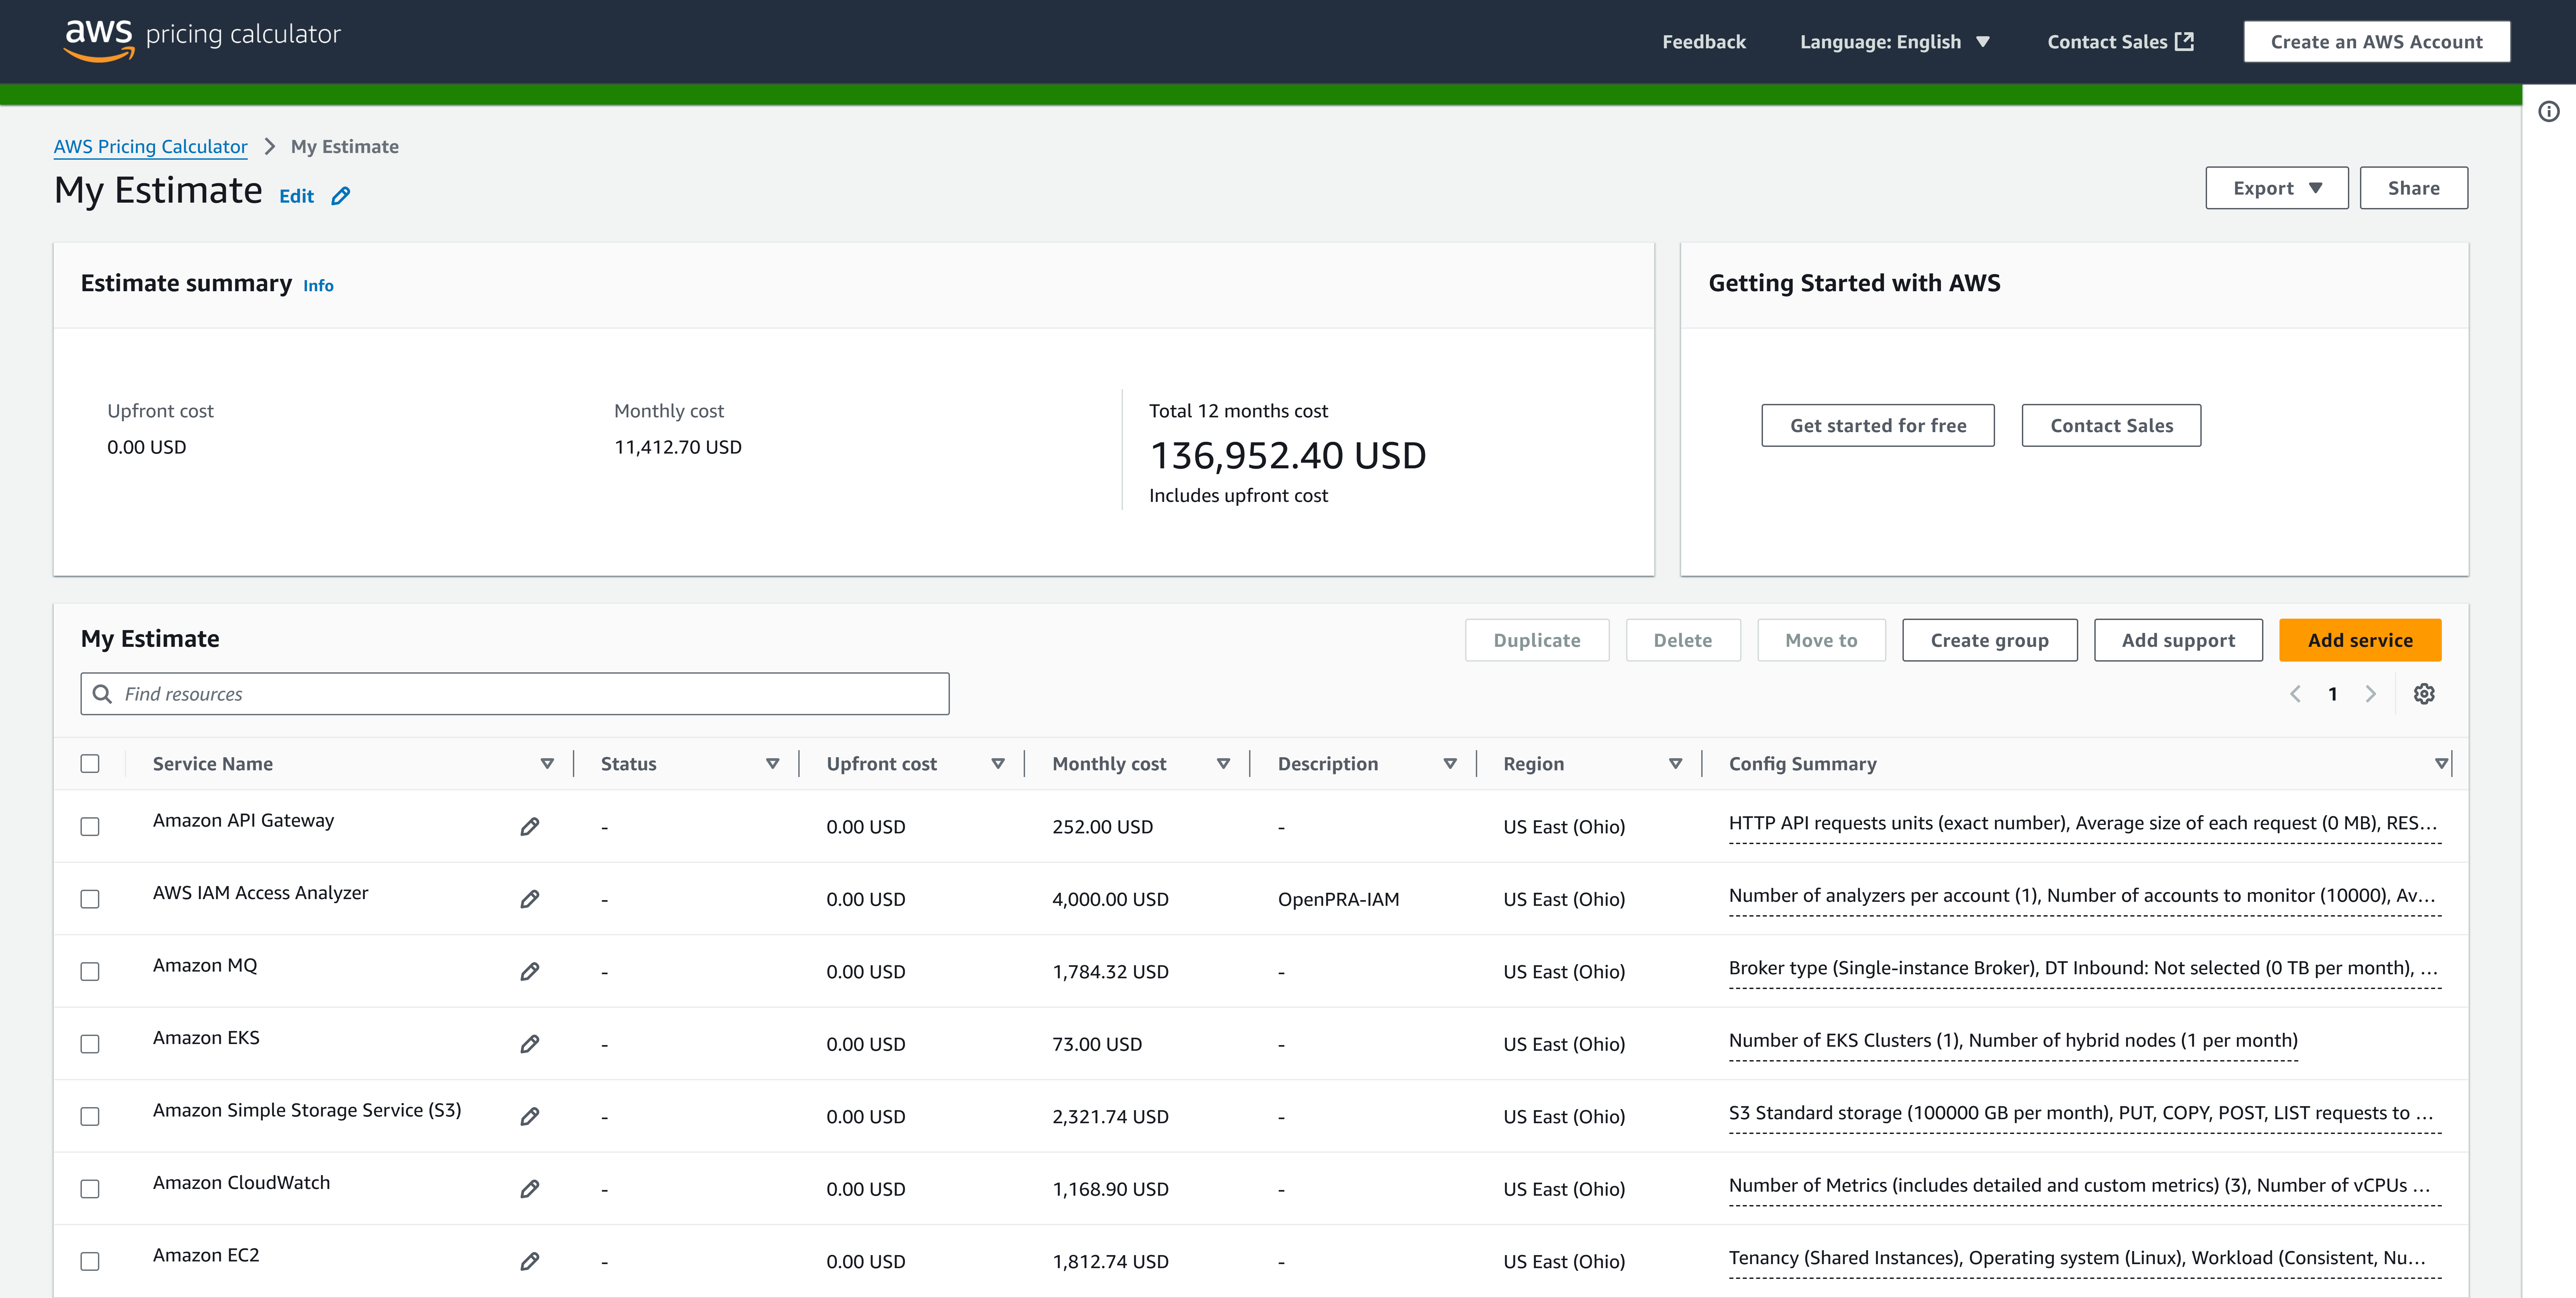
\includegraphics[width=1.1\textwidth]{6-experimental-evaluation/figures/aws_calculator.png}
  \caption{Estimated pricing for the cloud based deployment.}
  \label{fig:aws_calculator}
\end{figure}

\iffalse

Because all event trees could be quantified easily with a truncation limit of \(10^{-12}\), the limit was tightened to \(10^{-20}\) to impose greater computational strain on the solvers and this approach succeeded. SAPHSOLVE was unable to quantify the ATRS and PCL event trees at \(10^{-20}\) within a 48 hour time window. SCRAM took up to 1.78 and 7.22 hours respectively, for the same limit. The execution runtimes and memory usage for the remaining five event trees at \(10^{-20}\) are shown in Figs.~\ref{fig:execution_runtime_1e-20} and \ref{fig:memory_usage_1e-20}, and these single node results define the performance target for the distributed system. Although distributed performance is reported for all trees at truncation limits of both \(10^{-12}\) and \(10^{-20}\), particular attention is focused on the ATRS and PCL event trees at \(10^{-20}\).

\subsection{Distributed Execution}

Because SCRAM’s C++ functions are wrapped as Node.js addons to expose them to the HTTP interface, SCRAM-node incurs substantial overhead compared to native SCRAM-cpp. Each request requires mapping JSON input into C++ objects, converting C++ results back to JSON, writing intermediate results to temporary files, and then streaming those files to MinIO object storage. The N-API bindings, serialization/deserialization, and file I/O all add latency to the overall quantification time.

Additional overhead arises from the way event trees are decomposed. For distributed quantification, the event tree is split into unique event sequences; each worker receives all data required to quantify a single sequence in isolation. Every time a worker processes a sequence, it must construct a separate PDAG, and no data structures are shared across workers. There is therefore no opportunity to cache intermediate results between sequences; each sequence is effectively quantified from scratch, and all of the aforementioned overheads are incurred for each one. The total processing time could be reduced if a caching mechanism were available to reuse partial results across sequences or workers.

These effects are visible in the performance results for a truncation limit of \(10^{-12}\) (Figs.~\ref{fig:distributed_mcub_runtime_1e12} and \ref{fig:distributed_rea_runtime_1e12}). With only two workers, the distributed configuration is slower than serial SCRAM-cpp in almost all cases: the per-sequence overhead dominates any benefit from parallelism. Once the number of workers is increased (4, 8, 16, 32, 64), the event sequences are parallelized more aggressively, and the net execution time begins to improve. Even then, for most of the smaller event trees the overhead of decomposition and data movement is still too large to offset the advantages of shared data structures and in-memory reuse in the serial solver.

A different picture emerges for the larger models at a truncation limit of \(10^{-20}\). As shown in Figs.~\ref{fig:distributed_mcub_runtime_1e20} and \ref{fig:distributed_rea_runtime_1e20}, the ATRS and PCL event trees take roughly 2~hours and 8~hours, respectively, to complete in serial SCRAM. However, profiling shows that only about 200~s (ATRS) and 400~s (PCL) are spent on the actual quantification; the remainder of the time is consumed by report generation, where SCRAM writes a single, very large output file.

In contrast, the distributed system benefits from the decomposed representation. Each event sequence produces its own partial report, and the final aggregation step extracts only the required fields and merges them efficiently. For ATRS and PCL at \(10^{-20}\), the distributed system completes report generation in approximately 330~s and 445~s, respectively which are close to the underlying quantification times. In these large-report cases, the distributed architecture not only matches but effectively “rescues” the performance that would otherwise be dominated by monolithic report writing in the serial solver. For the other five event trees, however, the problems are not large enough for these advantages to outweigh the overhead of decomposition, serialization, and network I/O, so serial SCRAM remains faster even with 64 workers.

Beyond raw performance, the main strength of the distributed architecture is its resilience and reliability for long running PRA tasks. In a serial workflow, the solver typically writes a single report only after the entire event tree has been quantified. If the solver or host fails mid-run, all progress is lost and the analysis must be restarted from the beginning. In the distributed system, progress is tracked per event sequence and persisted via the HTTP service and object storage. Individual worker failures or node outages do not halt the entire run; only the affected sequences need to be resubmitted. Moreover, failed sequences can be selectively re-executed with modified parameters (e.g., relaxed truncation thresholds) to obtain approximate results, and those results can be merged back into the overall analysis. This enables progressive, fault tolerant quantification for large scale PRA without requiring complete restarts after every failure.

\section{Summary}

From the case study, several points are clear:

\begin{itemize}
  \item The distributed system is well suited to long running quantifications that must complete reliably, even in the presence of partial failures or node outages.
  \item It is particularly effective for bulk and batch workloads, where many event trees or sequences can be submitted and processed concurrently.
  \item It supports use cases where users do not need immediate results and can submit jobs asynchronously, allowing the system to execute them to completion in the background.
  \item For very large models where report generation dominates runtime, the decomposed, per-sequence reporting strategy of the distributed system can significantly reduce end-to-end execution time compared to monolithic serial report writing.
\end{itemize}

\fi

%\section{Source Code Listings}
%\section{Configuration Files}
%\section{Experiment Scripts}
%\subsection{Hardware and Software Environment}
%\subsection{Test Models and Workloads}


%\section{Experiment 1: Serialized vs Parallel vs Distributed Execution}
%\section{Experiment 2: Speedup for Different Models}
%\section{Experiment 3: Speedup for Different Calculation Types}
%\section{Experiment 4: Speedup vs Number of Workers/Nodes}
%\section{Experiment 5: Priority Queue Handling (Mixed Job Types)}
%\section{Experiment 6: Overhead Analysis (Small, Medium, Large Models)}
%\section{Experiment 7: System Metrics (Latency, Throughput, Error Rate)}


%\begin{figure}[]
  \centering
  \includesvg[width=\textwidth]{6-experimental-evaluation/figures/distributed_mcub_runtime_1e12.svg}
  \caption{Runtime for serial vs distributed execution of SCRAM and SAPHSOLVE for MCUB approximation across seven event tree models (lower is better) for a truncation limit of $10^{-12}$.}
  \label{fig:distributed_mcub_runtime_1e12}
\end{figure}
%\input{6-experimental-evaluation/plots/distributed_rea_runtime_1e12}
%\input{6-experimental-evaluation/plots/distributed_mcub_runtime_1e20}
%\begin{figure}[]
  \centering
  \includesvg[width=\textwidth]{6-experimental-evaluation/figures/distributed_rea_runtime_1e20.svg}
  \caption{Runtime for serial vs distributed execution of SCRAM and SAPHSOLVE for REA approximation across seven event tree models (lower is better) for a truncation limit of $10^{-20}$.}
  \label{fig:distributed_rea_runtime_1e20}
\end{figure}